\section{Motivation}\label{sec:motivation_md_2022}
As discussed in the previous chapter, PyHEADTAIL simulations including the SPS impedance model suggest that the beam coupling impedance leads to an effective suppression of the $\CC$ RF phase noise induced emittance growth through the separation of the coherent tune from the incoherent spectrum. This emittance growth suppression, which is related to the coherent (dipole) motion, can reach up to a factor of 4-5 for the experimental conditions of the first experimental campaign with $\CC$s that took place in the SPS in 2018, and seems to be the explanation for the experimental observations (see Section~\ref{sec:MD5_overview}).

This emittance growth suppression effect has not been observed before. To this end, another experimental campaign took place in the SPS in 2022 where the main objective was to validate experimentally the above-mentioned suggested emittance growth suppression mechanism. If successful, it would constitute the first experimental investigation and validation of this effect. Moreover, achieving a good understanding of the 2018 results is essential for developing confidence in the theoretical model and its predictions for the HL-LHC.

The experimental campaign of 2022 was organised in five experiments which aimed to investigate in the SPS machine the effect of the imepdance on the noise-induced emittance growth. The first four experiments were carried out with artificial noise injected in the $\CC$ RF system. The fifth expereiment took place with a pure dipolar noise source: the beam transverse damper. This chapter reports on the preparation, the methodology, and the results of these experiments.

%The experimental campaign of 2022 was organised in two proof-of-concept experiments. The first experiment was carried out in the presence of phase noise in the $\CC$ RF system. The second experiment took place with a pure dipolar noise source: the beam transverse damper. This chapter reports on the preparation, the methodology, and the results of these experiments.


\section{Machine and beam configuration}\label{sec:cc_md_2022_parameters}
The emittance growth measurements in 2022 were performed in "coast" mode at 270\,GeV following the same setup as in 2018 (see Section~\ref{sec:exp_setup_2018}) and very similar machine and beam conditions. The most relevant parameters are listed in Table~\ref{tab:machine_beam_param_2022}. The listed values of the transverse normalised emittance, of the bunch length and of the intensity correspond to the requested intial values of each coast. The measured values of these parameters will be commented in the following sections and the detailed measurements throught the experiments are available in the Appendix~\ref{ch:app_measurments_22}. 

\begin{table}[!hbt]
	\begin{minipage}{\textwidth}
      \begin{centering}
   \caption{Main machine and beam parameters for the emittance growth studies in SPS in 2022.}
	\begin{tabu} to \textwidth {X[c,m] X[0.5c,m] X[0.5c,m] X[0.01c,m]}
		&&& \\[-6mm]
		\toprule \toprule
		\multicolumn{2}{l}{\textbf{Parameter}} &
		\multicolumn{2}{c}{\textbf{Value}} \\
		\bottomrule
      \multicolumn{2}{l}{Beam energy, $\symE$} & \multicolumn{2}{c}{270\,GeV} \\
      \multicolumn{2}{l}{Main RF voltage / frequency,  $\VRF$ / $\fRF$}  & \multicolumn{2}{c}{5\,MV / 200.39\,MHz} \\ %200.3945
      \multicolumn{2}{l}{Horizontal / vertical betatron tune, $\Qx$ / $\Qy$}  & \multicolumn{2}{c}{26.13 / 26.18} \\
      \multicolumn{2}{l}{Horizontal / vertical first order chromaticity, $\Qpx$ / $\Qpy$}  & \multicolumn{2}{c}{  0.0-1.0 / 0.0-1.0} \\
      \multicolumn{2}{l}{Synchrotron tune, $Q_s$}  & \multicolumn{2}{c}{0.0051} \\
      \multicolumn{2}{l}{Number of protons per bunch, $\Nb$} & \multicolumn{2}{c}{3 $\times 10^{10}$ p/b$^\ast$} \\
      \multicolumn{2}{l}{Number of bunches}  & \multicolumn{2}{c}{1} \\
      \multicolumn{2}{l}{Bunch length, 4$\sigmat$}  & \multicolumn{2}{c}{1.83 \,ns$^\ast$}\\
      \multicolumn{2}{l}{Horizontal / vertical normalised emittance, $\emitx$ / $\emity$}  & \multicolumn{2}{c}{2\,$\mathrm{\mu m}$ / 2\,$\mathrm{\mu m^\ast}$}\\
      \multicolumn{2}{l}{Horizontal / vertical rms tune spread, $\Dqxrms$ / $\Dqyrms$}  & \multicolumn{2}{c}{1.9 $\times 10^{-5}$ / 2.1 $\times 10^{-5}$ $^\ddagger$}\\
      \bottomrule
      \multicolumn{2}{l}{$\CC 1$ voltage / frequency, $\CCvoltage$ / $\CCfrequency$}  & \multicolumn{2}{c}{1\,MV / 400.78\,MHz} \\
      \bottomrule
	\end{tabu}
   \label{tab:machine_beam_param_2022}
   \end{centering} \footnotesize{$^\ast$ These values corresponds to the requested intial values at the start of each coast.  \\$^\ddagger$ Here the rms betatron tune spread includes only the contribution from the detuning with amplitude present in the SPS machine. More details along with the calculations for the listed values can be found in Appendix~\ref{app:detuning_with_amplitude}.}
   \end{minipage}
\end{table}
% For bunch length: cernbox/2022/SPS_MDs_2022/cc_md_16May2022/longitudinal_profiles/visualise_pickle.ipynb

\textcolor{red}{This paragraph needs to be checked.}
The emittance growth measurements of 2018, indicated that the betatron coupling in the SPS was small but not zero. On this ground, for the experimental campaign of 2022, there was an effort to reduce the betatron coupling in the SPS. The betatron coupling correction was performed before the start of the emittance growth measurements on May 16, 2022, using the skew quadrupoles to minimse the tune signal from the horizontal (vertical) plane in the FFT measurements of the vertical (horizontal) plane. It is assumed that the settings of the skew quadrupoles remained unchanged for all of the five experiments.

On the grounds that the last three (out of four) bunches used in 2018 expereimental campain were unstable, in 2022 the experiment was carried out with a single bunch. This choice allowed also to have better control on the beam conditions, avoiding possible effects from interactions between the bunches~\footnote{Even though these effects should be insignificant due to the large bunch spacing, see Table~\ref{tab:machine_beam_param_2018}.}.

In the experimental campaign of 2018, $\CC$2 was used. In the contrary, in 2022 the experiments with  $\CC$ RF noise were conducted with $\CC$1 for reasons discussed in Section~\ref{subsec:cc_calibration_2022}.

Finally, the emittance values were measured with the SPS Wire Scanners according to the procedure discussed in Section~\ref{subsec:sps_ws}. In particular, Wire Scanners SPS.BWS.51637.H and SPS.BWS.41677.V were used for measurements in the horizontal and vertical planes, respectively. For both devices the data points from the second photomultiplier were used (PM2)~\footnote{Each Wire Scanner device is equipped with four PMs. Each one of them provides a better resolution of the amplitude signal of the secondary particles for a different regime. The choice of PM2 for the emittance growth studies in 2022 was done "online", during the experiment, by examining the obtained beam profiles.}. The beta functions of the respective plane at the locations of the wire scanners are 79.29\,m, and  60.75\,m. 
% The values of the beta functions were obtained from MADX: https://github.com/natriant/exploring_SPS/blob/master/madx_studies/optics_new_seq_after_LS2/output/twiss_thin_elements/find_beta_functions_at_locations.ipynb 
As explained earlier (see Section~\ref{subsec:sps_ws}) during each measurement with the wire scanners the beam profile is acquired two times as the wire crosses the beam in the forward direction (IN scan) and then, 200\,ms later, in the reverse direction (OUT scan). The analysis that is presented in this theis, consider only the IN scan measurements for reasons that are discussed in the Appendix~\ref{sec:sps_transverse_beam_profiles}.



\section{Preparatory studies with PyHEADTAIL simulations}\label{sec:preparatory_studies_2022_cc}

In preparation for the experiments with $\CC$, the emittance growth in the presence of $\CC$ RF phase noise was simulated with PyHEADTAIL including the most up-to-date SPS impedance model~\cite{updated_sps_wakfields_model} as a function of amplitude-dependent tune spread introduced by octupoles. In particular, the octupoles of the LOD family were considered as they act mostly in the vertical plane which is the plane of interest in this studies (vertical $\CC$ module which results in vertical emittance growth). The beam and machine parameters are the ones reported in Table~\ref{tab:machine_beam_param_2022} which correspond to the experimental conditions of 2022. These preparatory studies were used to identify different regimes of the phenomenon of the emittance growth suppression by the beam transverse imepdance for the experimental machine conditiones and served as a guide for the planning of the experiments.

The emittance growth is induced by $\CC$ RF phase noise with a power spectral density of 1.68\,$\mathrm{rad^2/Hz}$ in the first betatron sideband which results in an emittance growth rate of about 25\,nm/s. It should be highlighted that this noise level is much stronger than the levels of the injected artificial noise used in the experiment, in order for the growth to be easily observed in the simulation time of just 2.5\,s. Therefore, the goal of the experiments was to reproduce the simulated suppression factor and behavior only and not the exact numbers. Finally, the simulation setup and the $\CC$ RF phase noise were simulated as discussed in Chapter~\ref{Ch:suppression_impedance}. 

The emittance growth was simulated over a range of twenty one $k_\mathrm{LOD}$ values equally spaced from -28.2$\mathrm{/m^4}$ to +28.3$\mathrm{/m^4}$. Nevertheless, in the simulations, no actual octupolar elements were used in order to avoid the excitation of resonances as discussed in Section~\ref{sec:first_obs_suppression}. Instead, following the preceding PyHEADTAIL simulations, the effect of the Landau octupoles is introduced as a change in the phase advance of the individual particles depending on their individual actions and defined by the corresponding detuning coefficients. The study was performed for zero horizontal detuning coefficient, $\alpha_{xx}$=0 since the horizontal coefficient does not affect the vertical emittance growth assuming zero coupling between the two transverse planes. The values of the vertical, $\alpha_{yy}$, and the cross-term, $\alpha_{yx}$, coefficients were estimated using MAD-X~\cite{madx}.

Figure~\ref{fig:pyheadtail_cc_impedance_2022_md_octupole_current} illustrates the dependence of the $\CC$ RF phase noise-induced emittance growth on the octupoles strength, in the absence (blue) and the presence (orange) of the wakefields. The analytical prediction of the model Mastoridis--Baudrenghien is also given to facilitate the identification of the suppression factor from the impedance (horizontal black dashed line). As usual, in the absence of wakefields, there is a very good agreement between the simulation results and the theoretical predictions. In the presence of wakefields, the expected dependence on the tune spread appears. The rms tune spread values (shown on the secondary horizontal axis) are computed taking into account both the $\alpha_{{yy}}$ and $\alpha_{{yx}}$ coefficients using Eq.~\eqref{eq:rms_amplitute_detuning_3}.

% 1) Slides on computing the octupole current: https://docs.google.com/presentation/d/1VgGMqCevej4Eh7bjdGFSEPVI0zLxqB2S5FxLtFGhp2I/edit#slide=id.ge970b2a80a_0_16
The green and yellow areas indicate regimes where the octupoles require less than 200\,A and 400\,A respectively for their operation. The maximum operational current for the defocusing octupole family (LOD) in SPS is 400\,A. However, due to their planned continuous operation in multiple coasts, the LOD current should stay below 200\,A. The required current for the octupoles is computed from their strength, $k_\mathrm{LOD}$, using Eq.~\eqref{eq:I_vs_B3_relation_lof}


% /eos/user/n/natriant/pyheadtail_data/final_for_thesis/2022_conditions/CC1/deyRates_sps_270GeV_PN1e-8_400MHz_SPS_CC2_updatedWakes_y-plane_WakesOFF_vs_WakesON_new_QpxQpy0.5_6D_Nb5e5_intensity3e10Scan_vs_TuneSpreadvsExpectedSPS_octupole_current.png
\begin{figure}[!h] % Email communication with T. Levens on 8 November 2021.
   \centering         
   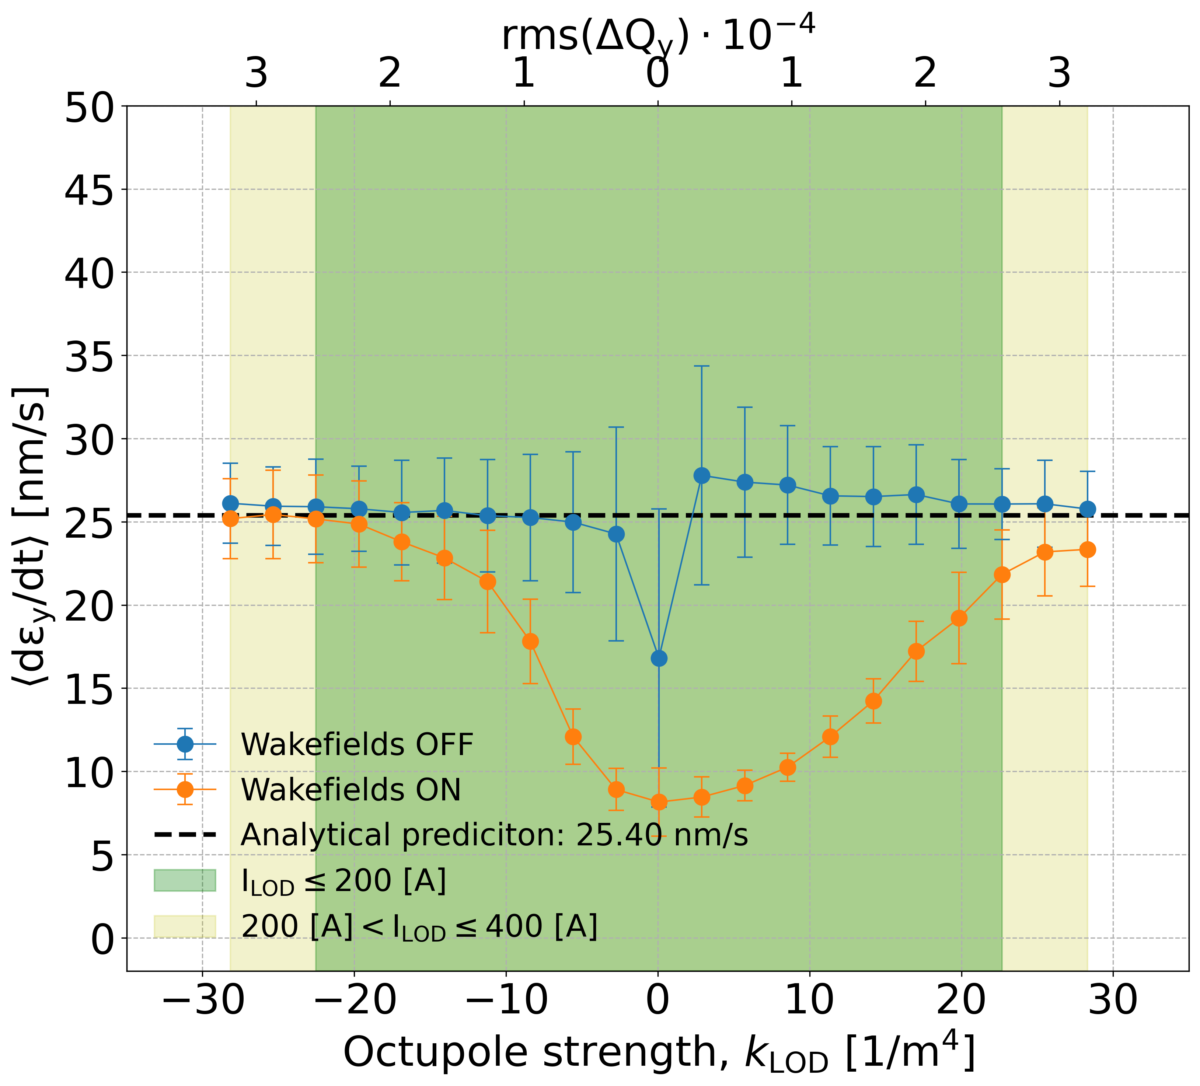
\includegraphics[width=0.8\textwidth]{images/Ch8/deyRates_sps_270GeV_PN1e-8_400MHz_SPS_NewWakesAllcontributions_appendWakes_y-plane_WakesONvsOFF_QpxQpy1_6D_Nb5e5_intensity3e10Scan_vs_TuneSpreadvsExpectedSPS_octupole_current.png}
       \caption{Transvserse emittance growth driven by CC RF phase noise without (blue) and with (orange) the impedance effects. The green and yellow areas indicate regimes where the octupoles require less than 200\,A and 400\,A respectively for their operation.}
       \label{fig:pyheadtail_cc_impedance_2022_md_octupole_current}
\end{figure}

From Fig.~\ref{fig:pyheadtail_cc_impedance_2022_md_octupole_current}, we make the following observations:
\begin{enumerate}
   \item For the octupoles switched off, $k_\mathrm{LOD}$=0, a suppression factor of about 3 is observed.
   \item The strong dependence of the emittance growth suppression on amplitude-dependent tune spread is observed for $k_\mathrm{LOD} \leq 20$\,$\mathrm{/m^4}$.
      \begin{itemize}
         \item The asymmetry in the suppression factor for positive and negative detuning with amplitude observed in the simulations for the 2018 experimental conditions (Chapter~\ref{Ch:suppression_impedance}) seems to be mitigated here. Nevertheless, the negative polarity of the octupoles (LOD) seems to slightly favor the exit the suppression region.
      \end{itemize}
   \item For $k_\mathrm{LOD} > 20$\,$\mathrm{/m^4}$ the emittance growth rate expected from Mastoridis--Baudrenghien model seemts to be restored. 
      \begin{itemize}
         \item Even for the strongest octupole strengths, $| k_\mathrm{LOD} |\approx 30 \ \mathrm{/m^4}$, the required current remains below 400\,A. Consequently, no crucial limitations are introduced to the experiment from the octupoles operation.
      \end{itemize}
\end{enumerate}

\section{Experiment I: dependence of Crab Cavity RF phase noise induced emittance growth rates on the noise power}\label{subsec:cc_md_2022_noise_scan} 

For the experiment described here, the emittance growth was measured in the presence of four different noise levels (as close as possible with the ones used in 2018) with the Landau octupoles switched off. The objective was a) to reproduce the scaling of emittance growth observed in 2018 (see Fig.~\ref{fig:MD5_summary_plot}) and b) to benchmark the expected suppression factor from PyHEADTAIL simulations with the impedance model. Experiment I took place in the SPS on May 16, 2022.

Four different levels of artificial noise were injected in the RF system of the $\CC$ as listed in Table~\ref{tab:noise_settings_2022} and the emittance evolution was recorded in coast mode every $\sim$1.5 minute. For each noise level, a new bunch was injected so that all measurements took place with the same initial conditions. The duration of each coast varied from about 30 minutes for the low noise levels to about 20 minutes for the strong noise. 

The linear chromaticity was corrected to about zero units in both the horizontal and vertical planes. That was a result of miscommunication with the operator team of the SPS machine as the desired value was between 0.5 and 1.0. However, the analysis of the PyHEADTAIL simulations in Section~\ref{subsec:chroma_scan} showed no significant sensitivity of the emittance growth suppression to the linear chromaticity values (for small positive values).

\subsection{Calibration of the Crab Cavity phase offset and voltage measurement}\label{subsec:cc_calibration_2022}

The first step before the emittance growth measurements, was to measure the $\CC$ voltage and calibrate the phase offset. It is reminded that in the experimental campaign of 2018, it was found that there was a phase offset between the set phase of the $\CC$ and the phase experience by the beam (see Section~\ref{subsec:CC_voltage_2018_measurement}). Even though simulation studies showed that for the long bunches used in the $\CC$ experiments the $\CC$ phase has no significant impact on the phase noise induced emittance growth~\cite{wp4_triantafyllou_2020} an automated procedure was developed for identifying and correcting this phase offset for completeness. The same procedure can also provide the amplitude of the $\CC$ voltage.

To provide an overview, the calibration was performed by varying the inspector phase of CC1 from -180$^\circ$ to +180$^\circ$ in steps of 30$^\circ$. For each step, the intra-bunch offset due to the $\CC$ was acquired with the Head-Tail monitor and the $\CC$ voltage signal was reconstructed following the same procedure described in Section~\ref{subsec:CC_voltage_2018_measurement}~\footnote{It is worth mentioning here that from the end of 2018 till the end of 2020, the CERN accelerator complex has undergone its second long shutdown in order to complete its scheduled upgrade program. Therefore, the calibration of the Head-Tail monitor which provides the normalisation factor that converts the measured intra bunch offset from arbitrary units to millimeters (more details in Appendix~\ref{subsec:HT_post_process_CC}) was repeated. The calibration factor for the Head-Tail monitor was measured to be 0.1037 in 2021(see Appendix~\ref{sec:HT_calibration_2022}).}. For each acquisition, the $\CC$ voltage at the center of the bunch, $t=0$, as it passes through the Head-Tail monitor was plotted as a function of the corresponding set value of the phase. The results of the phase scan for $\CC$1 are summarised in Fig.~\ref{fig:Vcc_calibration_md_2022} (blue dots). 
The three-parameter sinusoidal function of Eq.~\eqref{eq:sin_fit_cc} which provides the amplitude, the phase and the vertical offset of the signal ($A, \theta, d$) is used to fit the measured data.

%The results are fitted with the three-paramter sinusoidal function of Eq.~\eqref{eq:sin_fit_cc} which provides the amplitude, the phase and the vertical offset of the signal ($A, \theta, d$).


\begin{figure}[!h] % /eos/user/n/natriant/2022/SPS_MDs_2022/cc_md_16May2022/HT_monitor_phase_CC_offset_calibration
   \centering         
   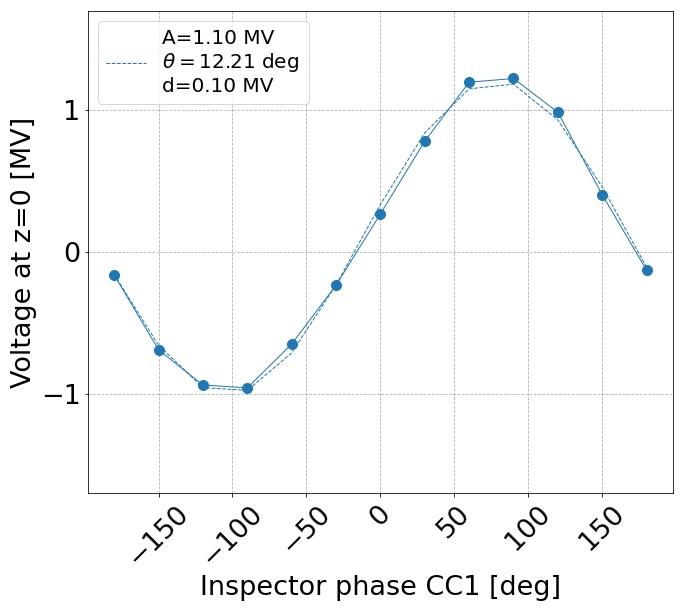
\includegraphics[width=0.7\textwidth]{images/Ch8/Vcc_at_z_zero_vs_inspector_phase_CC1_for_thesis.png}
       \caption{Calibration plot for the CC1 as obtained during the experiment on 16 May 2022, displaying the CC voltage at the center of the bunch $t=0$ for different phase values set in the CC.}
       \label{fig:Vcc_calibration_md_2022}
\end{figure}

The results of the sinusoidal fit (blue dashed line) are illustrated in the legend box in Fig.~\ref{fig:Vcc_calibration_md_2022}. Hence, it can be concluded that from the beam based measurements with the Head-Tail monitor the phase offset was found to be 12.21$^\circ$. For the rest of the experiment, the inspector phase was set to the opposite of the phase offset so that the phase of the $\CC$ voltage experienced by the bunch is zero. 


From the fit the amplitude voltage of CC1 was found to be (following the discussion in Section~\ref{subsec:CC_voltage_2018_measurement}): $\CCvoltage=A \pm d = 1.1 \pm 0.1$\,MV, very close to the targeted one (1\,MV). This approach of measuring the $\CC$ voltage experienced by the beam is preferred over the approach used in 2018, since now multiple Head-Tail acquisitions are taken into account in contrary with the single acquisition used in 2018.  


%since now the amplitude is obtained from a sinusoidal fit over multiple Head-Tail acquisitions while in 2018, only one acquisition was used.

For reference, the calibration for $\CC$1 took place at 270\,GeV and it lasted for about 15 minutes (start: $\sim$09:40, end: $\sim$09:52).

Between $\sim$11:39 and $\sim$11:45 the same scan for CC2 was attempted. However, the cavity tripped systematically due to issues associated with the change of the RF phase. Fixing this issue would have been time-consuming, and was not possible due to the very limited machine time for the experiment. Therefore, for the measurements in 2022 $\CC$1 was used.
% CC2 tripped: see the entry of the logbook 4/5/2022, at 11:30:30 


\subsection{Measurement of background growth rate in "coast" mode}\label{subsec:measured_background_growth_cc_md_2022}
After the calibration of $\CC$1, the coast at 270\,GeV was set up for the emittance growth measurements. First, the background emittance growth, with no additional noise injected in the CC and the Landau octupoles switched off was measured. The background emittance growth was found to be similar in both transverse planes: $d\epsilon_x /dt$ = 0.81\,$\mathrm{\mu m}$ and $d\epsilon_y /dt$ = 0.84\,$\mathrm{\mu m}$ in the horizontal and vertical planes respectively. This measured background emittance growth is illustrated in Fig~\ref{fig:cc_md_2022_background_growth_in_scan} for both the horizontal (blue) and vertical (red) planes.

\begin{figure}[!h] % /eos/user/n/natriant/2022/SPS_MDs_2022/cc_md_16May2022/roundA_online_analysis_ws/online_analysis_scripts_figures/coast1
   \centering         
   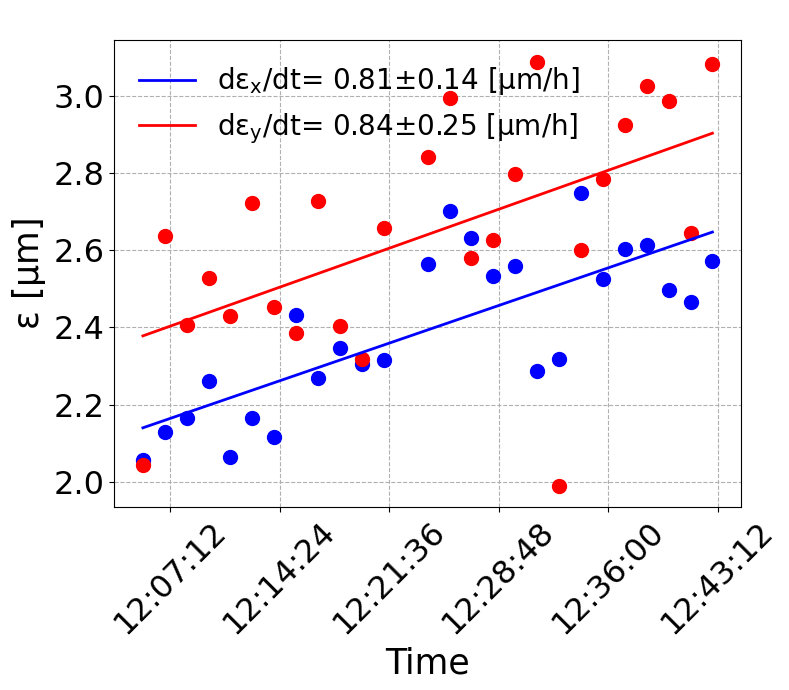
\includegraphics[width=0.7\textwidth]{images/Ch8/cc_md_2022_background_in_scan.png}
       \caption{Horizontal (blue) and vertical (red) background emittance growth measured during the experiment with CC1 on May 16, 2022, with no artificial noise injected in the CC RF system and with the Landau octupoles switched off.}
       \label{fig:cc_md_2022_background_growth_in_scan}
\end{figure}
% There was no valid reason to exclude any of the points even the outliers.

The applications used in the control room for the monitoring of the SPS machine have undergone an upgrade between the years 2018 and 2022. The latest applications which activate the wire scanners and automatically compute the emittance values from the profiles do not compute the respective errors. Nevertheless, the profile measurement data are available and thus the uncertainties of the emittance values can be calculated at a later post-processing stage. This post-processing showed that the uncertainties of the emittance values (computed as shown in Chapter~\ref{Ch:2018_analyisis}) are 2-3 orders of magnitude smaller than the emittance values themselves (see Appendix~\ref{sec:sps_transverse_beam_profiles}). Therefore, their impact is insignificant and the uncertainties of the emittance growth rates are dominated by the fluctuation of the Wire Scanner acquisitions. To this end, they are not shown in the emittance growth plot nor included in the fit to facilitate the [post-processing.

From the above figure, it is evident that there is a significant fluctuation in the emittance values in both transverse planes. By looking at the beam profiles, no evidence (e.g. corrupted profiles, abnormal tails, large errors on the gaussian fit results) was found to exclude some of the points. This fluctuation is introduced by the Wire Scanners used for the measurements. As discussed with the experts it appears to be within the limitations of the instrument for these small emittance values. In order to reduce the sensitivity of the linear fit (from which the emittance growth rates are obtained) longer measurements are required (at least 40 minutes). For larger emittance growth rates, or in other words for larger emittance values, the effects of the fluctuations are mitigated.

Finally, for reference, the noise floor of the amplitude and phase noise of the $\CC$ at 8\,kHz were measured to be -130.2\,dBc/Hz and 125.7\,dBc/Hz respectively. From the Mastoridis--Baudrenghien model the expected emittance growth from those noise levels was 0.08\,$\mathrm{\mu m/h}$ and 0.2\,$\mathrm{\mu m/h}$ in the horizontal and vertical planes respectively from both noise types combined. These analytically computed rates were obtained for bunch length, $4\sigma_t=1.83$\,ns and the measured amplitude of the $\CC$ voltage of $\CCvoltage=1.1$\,MV.
% y-plane --> AN: 0.05 um/h, PN: 0.15 um/h
% x-plane --> AN: 0.02 um/h, PN: 0.06 um/h
% Directory to compute these rates: /afs/cern.ch/work/n/natriant/public/SPS_MDs_2022/cc_md_16May2022/cmpt_emit_growth_theoretical_model
% Also some of the growth in the horizontal plane is expected by the IBS. How much I do not know yet.
The rest of the observed growth rates, is due to other sources which have not so far been identified (discussed in Chapter~\ref{Ch:2018_analyisis}).



\subsection{Injected Crab Cavity RF noise}\label{sec:injected_cc_noise_2022}
The noise injected in the $\CC$ RF system was a mixture of phase and amplitude noise up to 10\,kHz as in 2018 experimental campaign. Thus the noise, overlaps and primarly excites the first vertical betatron sideband only, at $\sim$~8\,kHz. The predicted transverse emittance growth from Mastoridis--Baudrenghien model can be computed using Eqs.~\eqref{eq:dey_an_sps} and~\eqref{eq:dey_an_sps} for amplitude and phase noise, respectively.

The power spectral density values at $\sim$~8\,kHz of the four different levels of artificial noise measured during the experiment are listed in Table~\ref{tab:noise_settings_2022} along with the corresponding expected emittance growth rates from the Mastoridis--Baudrenghien theory. By looking at the table, it is evident that the contribution of amplitude noise to the total emittance growth was found to be small: about 7~$\%$ on average over all noise settings.



%The noise excitation extended from DC up to about 10\,kHz and thus the noise was applied on the first vertical betatron sideband only, at $\sim$~8\,kHz. The power spectral density values at $\sim$~8\,kHz of the four different levels of artificial noise that were used in the experiment are listed in Table~\ref{tab:noise_settings_2022}. By looking at the table, it is evident that the contribution of amplitude noise to the total emittance growth was found to be small: about 7~$\%$ on average over all noise settings.

%By looking at the table, it becomes evident that the contribution of amplitude noise to the total emittance growth was found to be small (about 7~$\%$). To this end, in the post-processing of the 2022 data, the introduction of the effective phase noise (see Section~\ref{sec:injected_RF_noise}) is not required. In the following, the measured growth rates will be displayed as a function of the measured RF phase noise only. This choice is also justified by the fact that the objective of the 2022 experimental campaign with $\CC$s is to mainly reproduce the qualitative expected bahevior from the impedance and not the exact values. This is discussed further in the next sections of this chapter.

% I don't have the data to plot the spectra. Only screenshots in the logbook.


% Note 1: Noise level values from the logbook.
% Note 2: Analysis and percentages: /2022/SPS_MDs_2022/cc_md_16May2022/roundA_online_analysis_ws/summary_plots/for_thesis/cc_md_analysis_noise_scan_for_thesis.ipynb
\begin{table}[!hbt]
	\centering
   \caption{Phase and amplitude noise levels injected in the CC RF system for the Experiment I in 2022 along with the analytically expected growths. The listed noise values correspond to the power spectral density values at the first vertical betatron sideband, $f_b$, at $\sim$~8\,kHz. The analytical emittance growth rates were computed using Eq.~\eqref{eq:dey_an_sps} and~\eqref{eq:dey_pn_sps} for bunch length of $4\sigma_t$=1.83\,ns and the measured amplitude of CC voltage, $V_\mathrm{CC,0}$=1.1\,MV.}
	\begin{tabu} to \textwidth { X[c,m] X[c,m] X[c,m] X[c,m] X[c,m]}
		&&&& \\[-6mm]
		\toprule \toprule
		\multicolumn{1}{l}{} &
		\multicolumn{2}{c}{$\mathbf{10\,\boldsymbol{\log}_{10} \mathcal{L}(f)}$ \textbf{[dBc/Hz]}} & \multicolumn{2}{c}{\textbf{Analytical } $\mathbf{d \boldsymbol{\epsilon}_y/dt \ [\boldsymbol{\mu} m/h]}$} \\
		\bottomrule
      \multicolumn{1}{l}{} & 	\multicolumn{1}{c}{\textbf{Phase noise}} & \multicolumn{1}{c}{\textbf{Amplitude noise}} & \multicolumn{1}{c}{\textbf{Phase noise}} & \multicolumn{1}{c}{\textbf{Amplitude noise}} \\
      \midrule
      \multicolumn{1}{l}{Level 1}  & \multicolumn{1}{c}{-115.2} & \multicolumn{1}{c}{-124.6} & \multicolumn{1}{c}{1.99} & \multicolumn{1}{c}{0.2} \\
      
      \multicolumn{1}{l}{Level 2}  & \multicolumn{1}{c}{-109.5} & \multicolumn{1}{c}{-120.5} & \multicolumn{1}{c}{7.39} & \multicolumn{1}{c}{0.51}\\

      \multicolumn{1}{l}{Level 3}  & \multicolumn{1}{c}{-104.7} & \multicolumn{1}{c}{-116.0} & \multicolumn{1}{c}{22.32} & \multicolumn{1}{c}{1.44} \\

      \multicolumn{1}{l}{Level 4}  & \multicolumn{1}{c}{-100.1} & \multicolumn{1}{c}{-111.0} & \multicolumn{1}{c}{64.35} & \multicolumn{1}{c}{4.54} \\ 
      \arrayrulecolor{black}\bottomrule
	\end{tabu}
   \label{tab:noise_settings_2022}
\end{table}


\subsection{Transverse emittance growth measurements}\label{sec:cc_md_2022_exp1}
Four different levels of artificial noise were injected in the RF system of the $\CC$ as listed in Table~\ref{tab:noise_settings_2022} and the emittance evolution was recorded in coast mode at 270\,GeV every $\sim$1.5 minute. For each noise level, a new bunch was injected so that all measurements took place with the same initial conditions. The duration of each coast varied from about 30 minutes for the low noise levels to about 20 minutes for the strong noise. 

For the strong noise, less measurement time is sufficient since the growth rate obtained from the linear fit on the emittance values is less sensitive to the fluctuations in the wire scanner measurements. Additionally, for strong noise, the emittance reaches very quickly very large values, about 8-10\,$\mathrm{\mu m}$, which eventually degrades the quality of the beam.

For reference, the transverse emittance growth measurements lasted for about 2.5\,hours (start: $\sim$12:50, end: $\sim$15:18).

Figure~\ref{fig:cc_md_2022_overview_plots_noise_scan} illustrates the transverse emittance growth measured during Experiment 1 in 2022 for the four different noise levels injected in the $\CC$ RF system increasing from top left to bottom right. These measurements are summarised in Fig.~\ref{fig:H_V_emit_growth_noise_scan} which gives an overview of the vertical and horizontal emittance growth rates plotted as a function of the four different phase noise levels. 

There is a clear emittance growth in the vertical plane which is faster for stronger noise as expected. A growth in the horizontal emittance is also observed, but this appears to be independent of the growth in the vertical. This indicates that the use of the skew quadrupoles (discussed in Section~\ref{sec:cc_md_2022_parameters}) sufficiently minimsed the betatron coupling. Consequently, even though in the 2018 analysis the total emittance growth given by $d\epsilon_y/dt +d\epsilon_x/dt $ was considered to account for effects of betatron coupling, in the 2022 analysis the growth in the horizontal and vertical planes will be treated separately.


% Note 1, figures: /eos/user/n/natriant/2022/SPS_MDs_2022/cc_md_16May2022/roundA_online_analysis_ws/for_thesis
% Note 2, scripts to plot: /afs/cern.ch/work/n/natriant/public/SPS_MDs_2022/cc_md_16May2022/ws_measurements 
\begin{figure}[htp]
   \centering
   \begin{subfigure}{.45\textwidth}
       \centering
       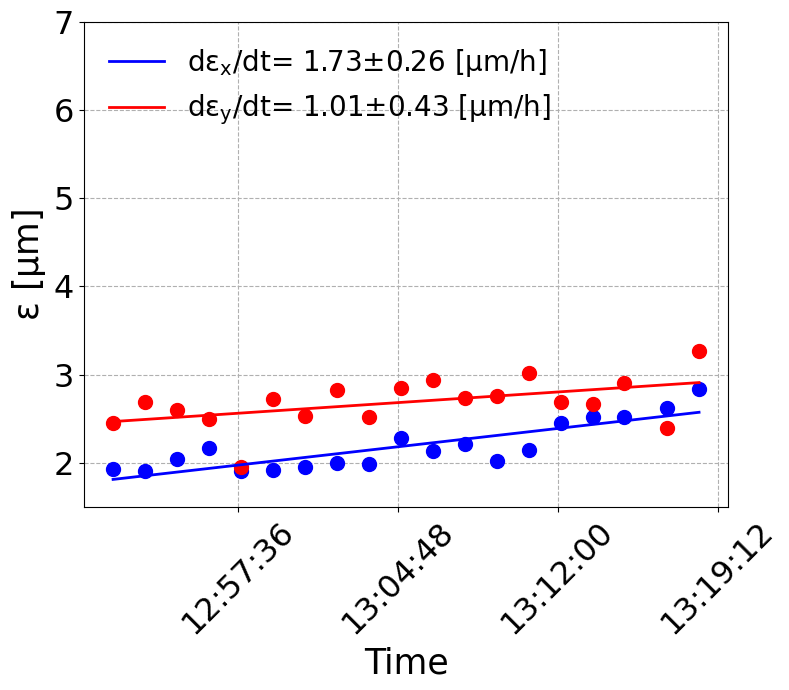
\includegraphics[width=.95\linewidth]{images/Ch8/emit_vs_time_Set1_coast2.png}  
       \caption{-115.2\,dBc/Hz}
       \label{fig:cc_md_2022_coast2}
   \end{subfigure}
   \begin{subfigure}{.45\textwidth}
       \centering
       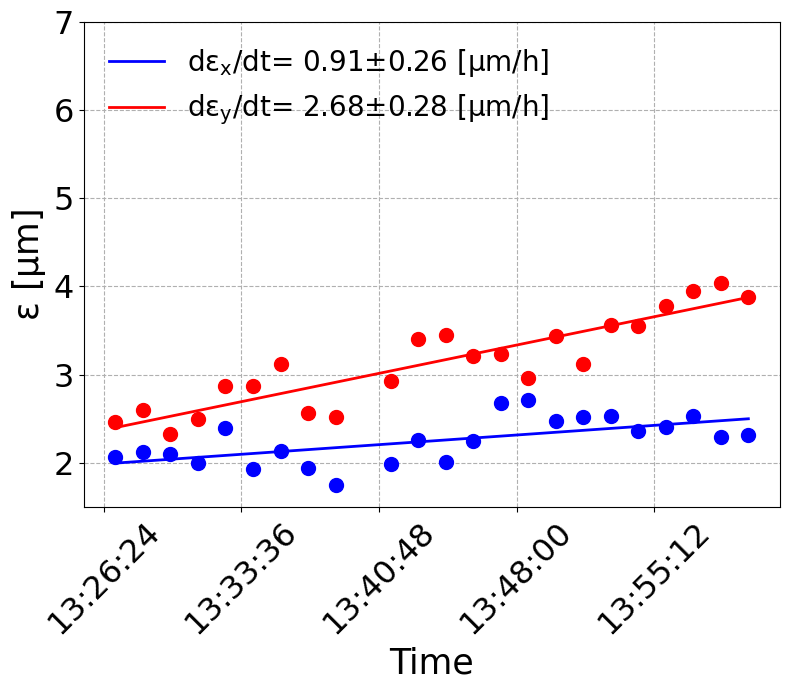
\includegraphics[width=.95\linewidth]{images/Ch8/emit_vs_time_Set1_coast3.png}  
       \caption{-109.5\,dBc/Hz}
       \label{fig:cc_md_2022_coast3}
   \end{subfigure}
   \begin{subfigure}{.45\textwidth}
       \centering
       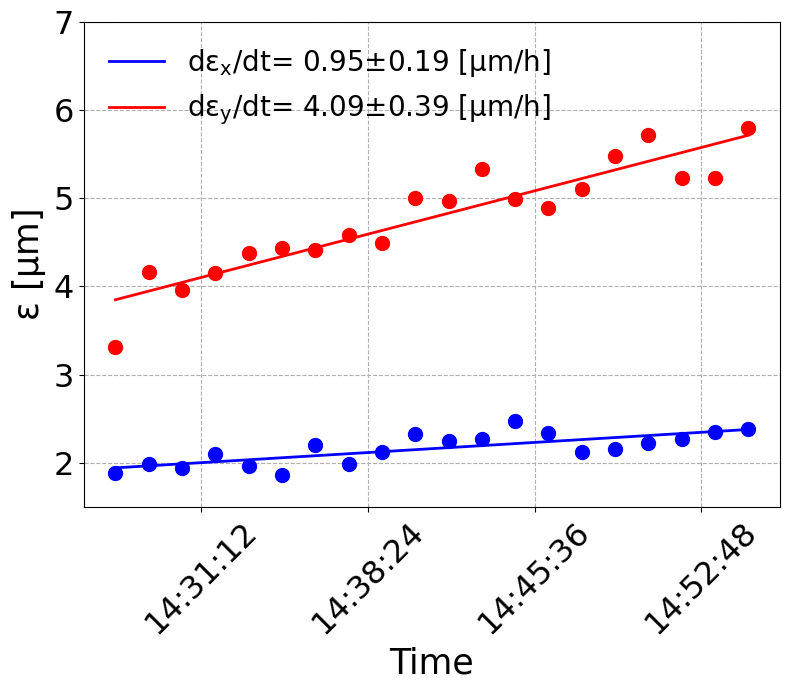
\includegraphics[width=.95\linewidth]{images/Ch8/emit_vs_time_Set1_coast4.png}  
       \caption{-104.7\,dBc/Hz}
       \label{fig:cc_md_2022_coast4}
   \end{subfigure}
   \begin{subfigure}{.45\textwidth}
           \centering
           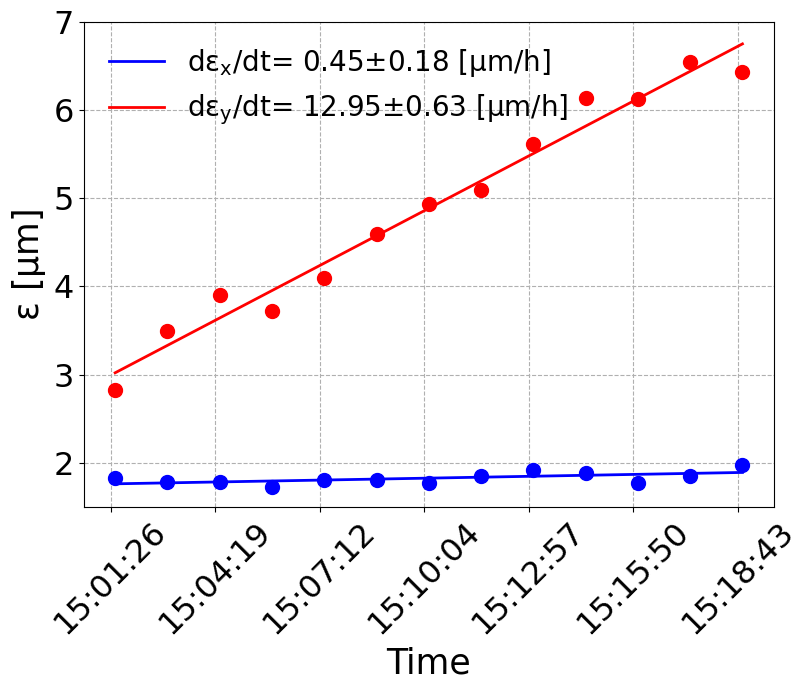
\includegraphics[width=.95\linewidth]{images/Ch8/emit_vs_time_Set1_coast5.png}  
           \caption{-100.1\,dBc/Hz}
           \label{fig:cc_md_2022_coast5}
   \end{subfigure}
   \caption{Horizontal (blue) and vertical (red) emittance evolution of a single bunch during Experiment I on 16 May, 2022. The different phase noise levels injected in the RF system of CC1, are shown in the caption for each plot.}
   \label{fig:cc_md_2022_overview_plots_noise_scan}
\end{figure}

% Figure: /eos/user/n/natriant/2022/SPS_MDs_2022/cc_md_16May2022/roundA_online_analysis_ws/summary_plots/for_thesis/emit_H_and_V_noise_scan.png
\begin{figure}[!h] 
     \centering         
   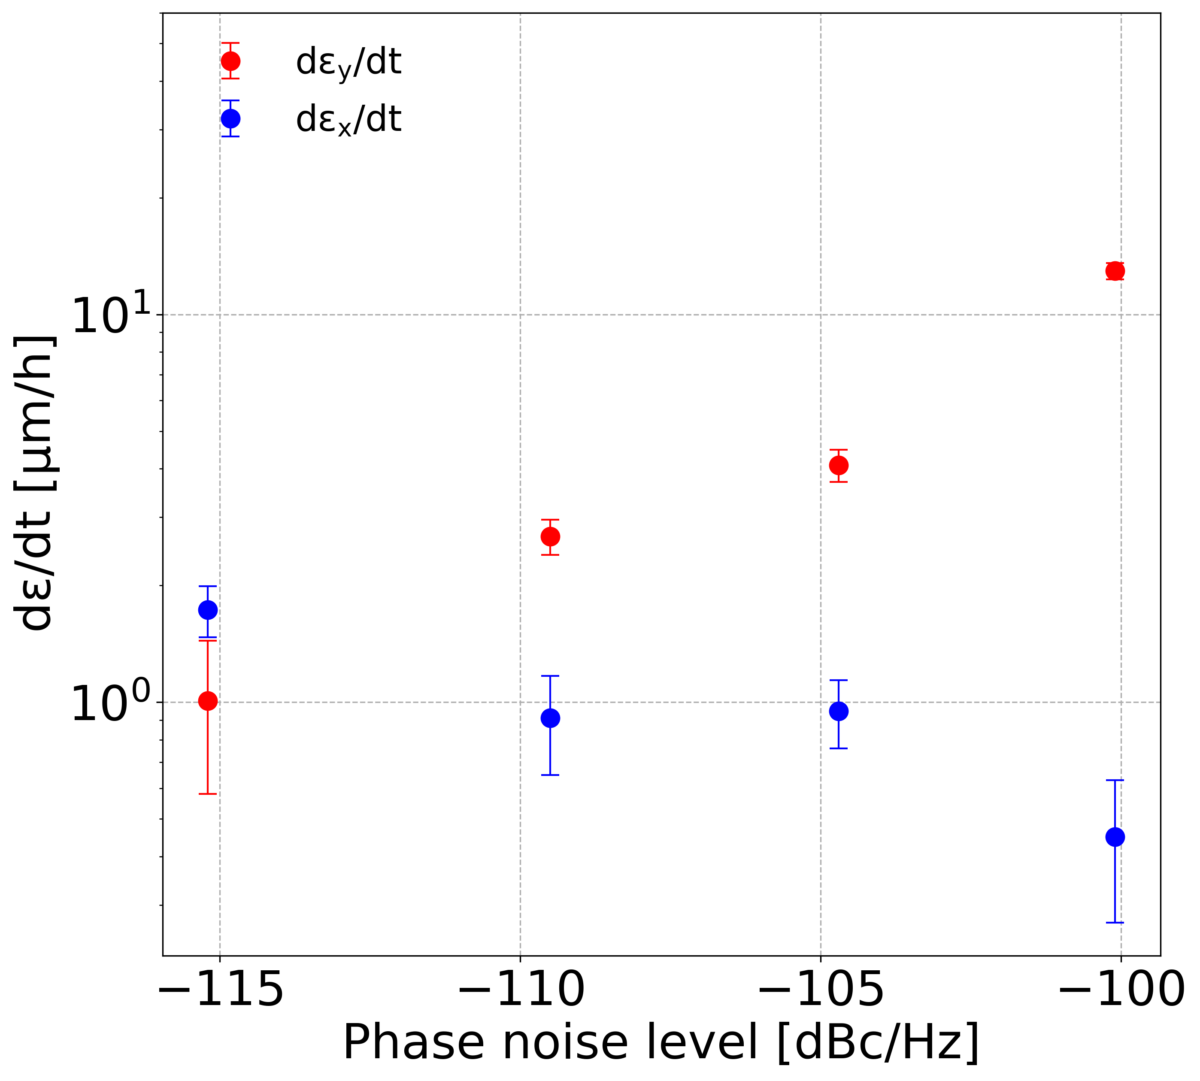
\includegraphics[width=0.7\textwidth]{images/Ch8/emit_H_and_V_noise_scan.png}
       \caption{Overview plot of the emittance growth study during Experiment 1 with noise injected in the CC1 in 2022. The measured horizontal (blue) and vertical (red) emittance growth rates are shown as a function of the different power levels of applied phase noise. The error bars indicate the error of the linear fit to the emittance values (see Section~\ref{sec:emit_growth_meas_2018}).}
       \label{fig:H_V_emit_growth_noise_scan}
\end{figure}

\subsection{Bunch length and intensity measurements}\label{sec:bunch_length_intensity_2022}

The bunch length measurements were performed with the Wall Current monitor. The bunch length evolution over each coastcan be found in Appendix~\ref{subsec:2022_exp1_bunch_length}. The average measured bunch length (over all coasts) was found to be about $4\sigma_t$ = 1.83\,ns. During the coasts, an increase in the bunch length of $\sim$5~$\%/h$ on average for each setting was observed. This small increase agrees with what is usually observed in the SPS in coast and will not be taken into consideration in the following analysis. 

%The individual plots illustrating the evolution of the bunch length as measured with the Wall Current Monitor (introduced in Section~\ref{sec:ABWLM_WallCurrentMonitor}) during the experiment are presented in Appendix~\ref{sec:bunch_length_measurements_2022}. Finally, looking at the dependence of the emittance growth suppression by the impedance on the bunch length in Fig.~\ref{fig:study_10_bunch_length} it is evident that the bunch length of $4\sigma_t$ = 1.83\,ns belongs to the regime of the strong suppression.

The intensity measurements were performed with the Beam Current Transformer (BCTDC) \textcolor{red}{add reference}. The bunch intensity over each coastcan be found in Appendix~\ref{subsec:2022_exp1_intensity}. The average intensity (over all coasts) was found to be about 2.9$\times 10^{10}$ protons per bunch, very close to the requested values of 3.0$\times 10^{10}$. No significantl, losses were observed during the coasts, therefore the evolution of the intensity is not considered in the following.

\subsection{Comparison of the transverese emittance growth with the predictions of Mastoridis--Baudrenghien theory}\label{sec:cc_exp1_2022_theory_vs_measurements}

%\textbf{Summary plot}\\
Figure~\ref{fig:V_emit_growth_background_subtracted_noise_scan} compares the measured (red) and the theoretically calculated (black) vertical emittance growth rates for the different noise levels. For the comparison the background growth rate measured in the vertical plane (see Section~\ref{subsec:measured_background_growth_cc_md_2022}) of 0.84\,$\mathrm{\mu m /h}$ is subtracted from the measured values. The subtraction of the background has practically no impact on the high noise levels but it is significant for the small ones. The concept of effective phase noise that was used in the analysis of the 2018 experimental date is not used here. The reason is that in 2022 we know that the effect of the emittance growth suppression that we are investigating does not have the same behavior in the presence of amplitude and phase noise. To this end, the horizontal axis displays the four different phase noise values since they were dominant. However, the theoretically calculated values are obtained by inserting both the phase and the corresponding ampitude noise levels of Table~\ref{tab:noise_settings_2022} in Eqs.~\eqref{eq:dey_pn_sps} and~\eqref{eq:dey_an_sps}, respectively, and for bunch length of $4 \sigma_t$ = 1.83\,ns, energy of 270\,GeV, the measured $\CC$ voltage amplitude $\CCvoltage=1.1$\,MV, and the vertical beta function at the location of $\CC$1, 76.07\,m.

%phase noise levels. For the comparison the background growth rate measured in the vertical plane (see Section~\ref{subsec:measured_background_growth_cc_md_2022}) of 0.84\,$\mathrm{\mu m /h}$ is subtracted from the measured values. The theoretically calculated values are obtained by inserting the phase and the corresponding ampitude noise levels of Table~\ref{tab:noise_settings_2022} in Eqs.~\eqref{eq:dey_an_sps} and~\eqref{eq:dey_pn_sps} and for bunch length of $4 \sigma_t$ = 1.83\,ns, energy of 270\,GeV, the measured $\CC$ voltage amplitude $\CCvoltage=1.1$\,MV, and the vertical beta function at the location of $\CC$1, 76.07\,m. The subtraction of the background has practically no impact on the high noise levels but it is significant for the small ones.

% Figure: /eos/user/n/natriant/2022/SPS_MDs_2022/cc_md_16May2022/roundA_online_analysis_ws/summary_plots/for_thesis/emit_V_background_subtracted_noise_scan_final.png
\begin{figure}[!h]
   \centering         
   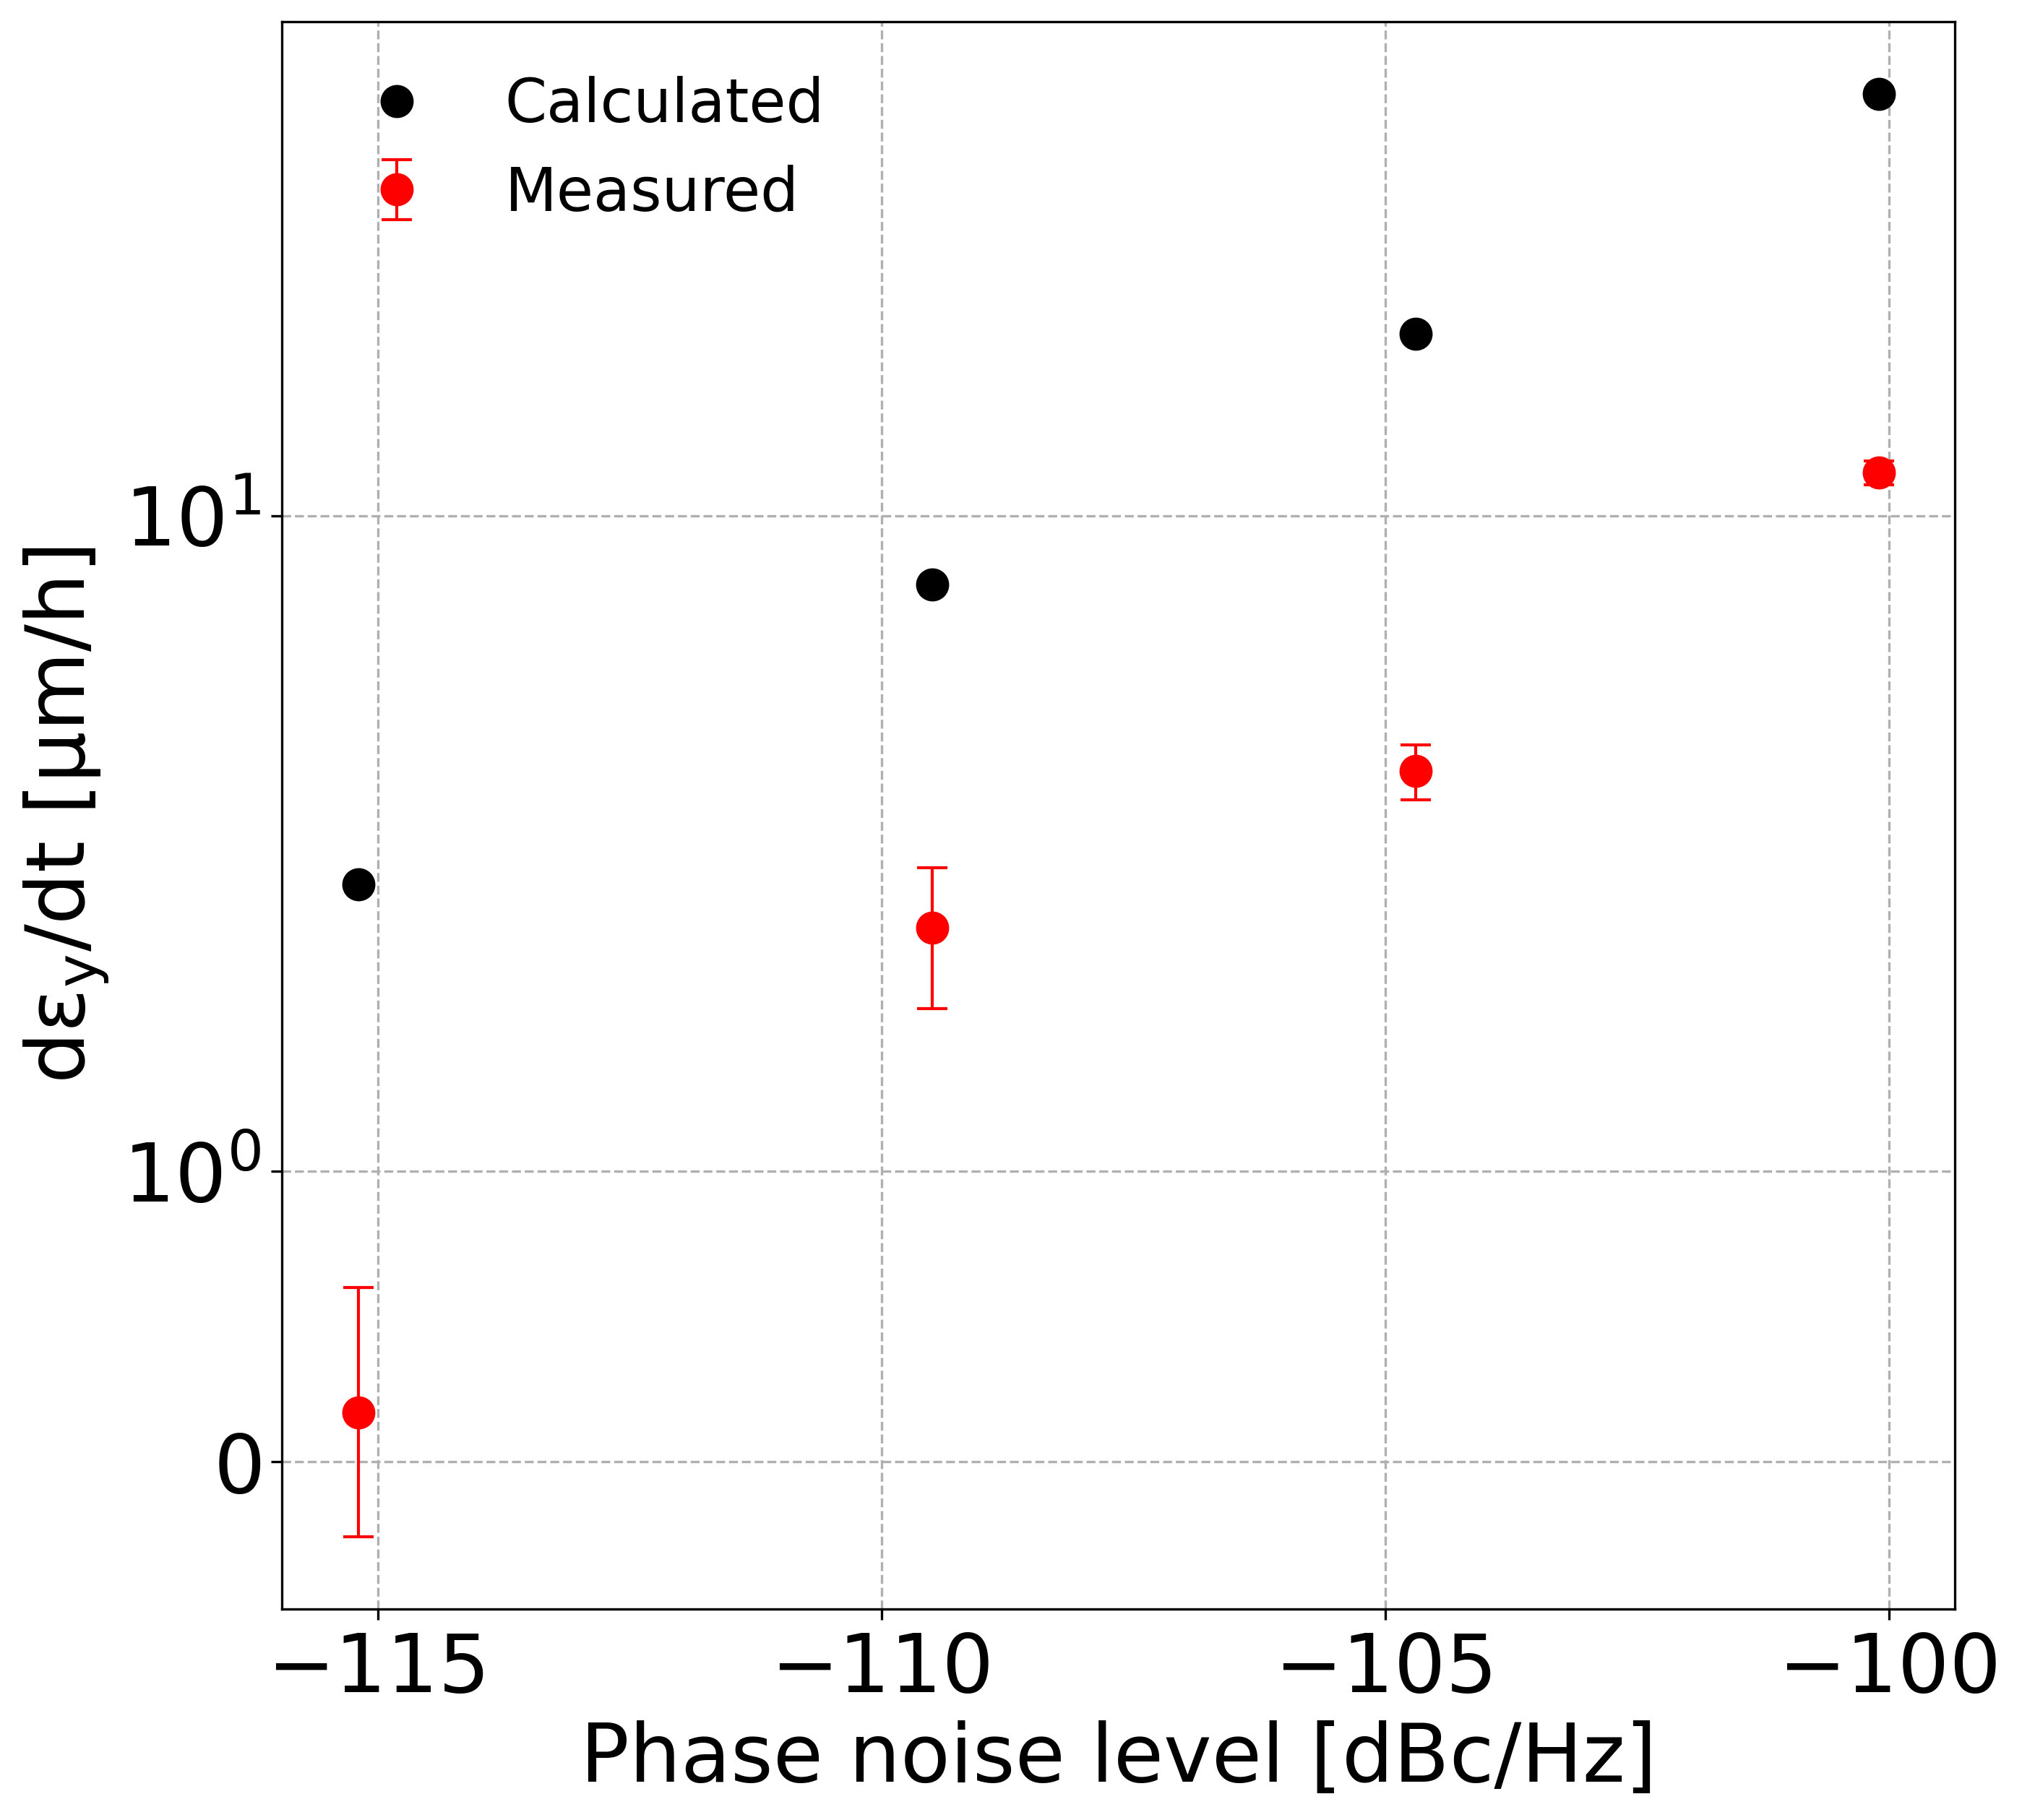
\includegraphics[width=0.7\textwidth]{images/Ch8/emit_V_background_subtracted_noise_scan_final.png}
       \caption{Summary plot of the emittance growth study with different noise levels injected in the RF system of CC1 during the Experiment I in 2022. The vertical measured growth rate (red) and the expected growths from the Mastoridis--Baudrenghien model (black) are shown as a function of the different levels of applied phase noise. The error bars indicate the error of the linear fit on the emittance values.}
       \label{fig:V_emit_growth_background_subtracted_noise_scan}
\end{figure}

From Fig.~\ref{fig:V_emit_growth_background_subtracted_noise_scan} it becomes evident that the measured emittance growth rate increases for higher noise levels as expected. Furthermore, it is observed that the theory systematically overestimates the growth rates. The averaged discrepancy over all noise levels, but the first one, is a factor of about 6: numerical values are given in Table~\ref{tab:cc_md_2022_noise_scaling}. In the computation of the average, the measured emittance growth rates for the first noise level is not included. For the first noise level the discrepancy between the measured emittance growth and the expected is a factor 12. However, the uncertainy on the measured emittance growth is very big ($\sim 50\%$ of the emittance growth rate itself).
% a factor of 4.3

%\begin{table}[!hbt]
%	\centering
 %  \caption{Comparison between the measured and the calculated transverse emittance growth rates for the different phase noise levels during the CC experiment of 2022. The analytical emittance growth rates were computed using Eq.~\eqref{eq:dey_pn} for bunch length of $4\sigma_t$=1.83\,ns and CC voltage, $V_\mathrm{CC,0}=1.1$\,MV. The background growth rate measured in the vertical plane of 0.84\,$\mathrm{\mu m/h}$ is subtracted from the measured values.}
%	\begin{tabu} to \textwidth { X[c,m] X[c,m] X[c,m] }
%		&& \\[-6mm]
%	   \toprule \toprule
%		\multicolumn{1}{c}{$\mathbf{10\,\boldsymbol{\log}_{10} \mathcal{L}(f)}$} &
 %     \multicolumn{2}{c}{\textbf{Growth rate [}$\mathbf{\boldsymbol{\mu}}$\textbf{m/h]}}  \\
		%\bottomrule
 %     \multicolumn{1}{c}{\textbf{[dBc/Hz]}} & \multicolumn{1}{c}{\textbf{\textbf{Measured}}} & \multicolumn{1}{c}{\textbf{Calculated}}  \\
 %     \midrule
%      \multicolumn{1}{c}{-115.2}  & \multicolumn{1}{c}{0.17} & \multicolumn{1}{c}{1.73} \\
      
 %     \multicolumn{1}{c}{-109.5}  & \multicolumn{1}{c}{1.84} & \multicolumn{1}{c}{6.42} \\

  %    \multicolumn{1}{c}{-104.7}  & \multicolumn{1}{c}{3.25} & \multicolumn{1}{c}{19.38}  \\

  %    \multicolumn{1}{c}{-100.1}  & \multicolumn{1}{c}{12.11} & \multicolumn{1}{c}{55.9}  \\ 
 %     \arrayrulecolor{black}\bottomrule
	%\end{tabu}
 %  \label{tab:cc_md_2022_noise_scaling}
%\end{table}

\begin{table}[!hbt]
	\centering
   \caption{Comparison between the measured and the calculated transverse emittance growth rates for the different phase noise levels during the Experiment I in 2022. This table is complementary of Table~\ref{tab:noise_settings_2022}.}
	\begin{tabu} to \textwidth { X[c,m] X[c,m] X[c,m] }
		&& \\[-6mm]
		\toprule \toprule
		\multicolumn{1}{c}{\textbf{Noise level}} &
      \multicolumn{2}{c}{\textbf{Growth rate [}$\mathbf{\boldsymbol{\mu}}$\textbf{m/h]}}  \\
		%\bottomrule
      \multicolumn{1}{c}{} & \multicolumn{1}{c}{\textbf{\textbf{Measured}}} & \multicolumn{1}{c}{\textbf{Calculated}}  \\
      \midrule
      \multicolumn{1}{c}{Level 1}  & \multicolumn{1}{c}{0.17} & \multicolumn{1}{c}{2.19} \\
      
      \multicolumn{1}{c}{Level 2}  & \multicolumn{1}{c}{1.84} & \multicolumn{1}{c}{7.9} \\

      \multicolumn{1}{c}{Level 3}  & \multicolumn{1}{c}{3.25} & \multicolumn{1}{c}{23.76}  \\

      \multicolumn{1}{c}{level 4}  & \multicolumn{1}{c}{12.11} & \multicolumn{1}{c}{68.9}  \\ 
      \arrayrulecolor{black}\bottomrule
	\end{tabu}
   \label{tab:cc_md_2022_noise_scaling}
\end{table}

To summarise, the Experiment I with different levels of CC RF noise injected in the CC RF system showed that:
\begin{itemize}
   \item The measured emittance growth was found to scale with the noise power as expected from the Mastoridis--Baudrenghien model. 
   \item The measured emittance growth rates were found to be systematically lower than the theoretically expected values. This observation is in accordance with the experimental observations of the 2018 campaign and validates the reproducibility of the experiment. 
   \item The fact that the vertical emittance growth was found to be lower than the predictions of Mastoridis--Baudrenghien model also shows a qualitative agreement with the PyHEADTAIL simualtions including the SPS imepdance model and the octupoles switched off (see Fig.~\ref{fig:pyheadtail_cc_impedance_2022_md_octupole_current} for $k_\mathrm{LOD}=0$). However, the discrepancy between measured and theoretically expected values was found to be about a factor of 6 which is twice the suppression factor of 3 which is expected from the PyHEADTAIL simulations.
\end{itemize}


\section{Experiment II: sensitivity of emittance growth rates to amplitude-dependent tune shift}\label{subsec:cc_md_2022_octupole_scan}

In Experiment II, the emittance growth driven by $\CC$ RF noise was measured for one noise level over a range of octupole (LOD family) strengths. The goal was to explore the regime for $k_\mathrm{LOD} \leq 20$\,$\mathrm{/m^4}$, where the dependence of the emittance growth suppression on the amplitude-dependend tune spread is expected to be strong (see Fig.~\ref{fig:pyheadtail_cc_impedance_2022_md_octupole_current}). Experiment II took place in the SPS on May 16, 2022, right after Experiment I, for the same beam and machine conditions. The measurements of the CC voltage and of the background emittance growth were not repeated since the values measured in Experiment I are also valid for Experiment II.

The experiment was performed by injecting artificial noise in the $\CC$ RF system. In particular, the emittance growth was driven by phase noise of -104.7\,dBc/Hz and by amplitude noise of -116.0\,dBc/Hz at $\sim$8\,kHz (Level 4 in Table~\ref{tab:noise_settings_2022}). 
% -104.7 dbc/Hz is about 3.4 * 10^{-11}.


\subsection{Transverse emittance growth measurements}\label{subsec:emit_growth_exp2}

In the limited time available for the experiment performing the full scan on the octupole strengths for $k_\mathrm{LOD} \leq 20$\,$\mathrm{/m^4}$ was not feasible. Only five octupole strengths could be used, $k_\mathrm{LOD} = \pm 5 \ \mathrm{m^{-4}}, 10 \ \mathrm{m^{-4}}$ and $15 \ \mathrm{m^{-4}}$. %The last value of octupole strength is expected to restore the growth rate to almost the values predicted by the Mastoridis--Baudrenghien model (approximately 20 $\mathrm{\mu m/h}$).
For each one of thee octupole strengths the bunch evolution was recorded for about 20 minutes by acquiring repeated Wire Scanner measurements and then performing a linear fit. For the measurements of each octupole strength a fresh bunch was used so that the initial conditions each time are as close as possible.

The individual measurements of the transverse emittance evolution for each octupole setting are shown in Fig.~\ref{fig:cc_md_2022_overview_plots_klod_scan}. Two main observations can be made. First, there is a clear sensitivity of the measured evolution of the vertical emittance to the octupole strength as expected from the PyHEADTAIL simualtions with the SPS transverse impedance model. The second observation is that a growth of $\sim 2-4 \ \mathrm{\mu m/h}$ is also observed in the horizontal plane. However, it does not seem to depend on the octupole strength. Both observations are also seen in the summary plot of Fig.~\ref{fig:H_V_emit_growth_background_subtracted_octupole_scan}.



PyHEADTAIL simulations with the SPS impedance model have revealed a significant sensitivity of the emittance growth suppression on amplitude-dependent tune shift (e.g. Fig.~\ref{fig:MD_2018_impedance_simulations}). This behavior can be tested experimentally in the SPS with the use of the Landau octupole families, which allow for the introduction of controlled detuning with amplitude. A successful reproduction of this behavior would provide the proof-of-concept for the emittance growth suppression mechanism from the beam transverse impedance. This will be referred to as $\CC$ Experiment B in the following. It should be mentioned, that for this experiment the octupoles of the LOD family are employed as they act mostly in the vertical plane which is the plane of interest in this studies (vertical $\CC$ module which results in vertical emittance growth).

\section{Experiment with CC as noise source}\label{sec:cc_md_2022}
Due to the preceding PyHEADTAIL simulations which provided strong evidence that the observed discrepancy between the 2018 measurements and the theoretical predictions could be explained by the beam transverse impedance additional machine time was dedicated to emittance growth studies with $\CC$ in the SPS in 2022. The time allocated for the $\CC$ experiment was limited to about 10 hours. Taking into consideration the time needed for the setup and the $\CC$ calibration the time available for the emittance growth measurements is reduced even more. To this end, measurement repeatability is limited and the experimental procedure had to be carefully planned in advance.
% Also you can add that each point in the emittance growth studies needs about 30-40 min.





\textbf{CC RF noise}\\
The noise injected in the $\CC$ RF system was again a mixture of phase and amplitude noise. The noise excitation extended from DC up to about 10\,kHz and thus the noise was applied on the first vertical betatron sideband only, at $\sim$8\,kHz. The power spectral density values at $\sim$8\,kHz of the four different levels of artificial noise that were used in the experiment are listed in Table~\ref{tab:noise_settings_2022}. By looking at the table, it becomes evident that the contribution of amplitude noise to the total emittance growth was found to be small (about 7$\%$). To this end, in the post-processing of the 2022 data, the introduction of the effective phase noise (see Section~\ref{sec:injected_RF_noise}) is not required. In the following, the measured growth rates will be displayed as a function of the measured RF phase noise only. This choice is also justified by the fact that the objective of the 2022 experimental campaign with $\CC$s is to mainly reproduce the qualitative expected bahevior from the impedance and not the exact values. This is discussed further in the next sections of this chapter.


\textbf{SPS Wire Scanners}\\
The emittance values were measured with the SPS Wire Scanners according to the procedure discussed in Section~\ref{subsec:sps_ws}. In particular, wire scanners SPS.BWS.51637.H and SPS.BWS.41677.V were used for measurements in the horizontal and vertical planes, respectively. For both devices the data points from the second photomultiplier were used (PM2) \footnote{Each Wire Scanner device is equipped with four PMs. Each one of them provides a better resolution of the amplitude signal of the secondary particles for a different regime. The choice of PM2 for the emittance growth studies in 2022 was done "online", during the experiment, by examining the obtained beam profiles.}. The beta functions of the respective plane at the locations of the wire scanners are 79.29\,m, and  60.75\,m. 
% The values of the beta functions were obtained from MADX: https://github.com/natriant/exploring_SPS/blob/master/madx_studies/optics_new_seq_after_LS2/output/twiss_thin_elements/find_beta_functions_at_locations.ipynb 

As explained earlier (see Section~\ref{subsec:sps_ws}) during each measurement with the wire scanners the beam profile is acquired two times as the wire crosses the beam in the forward direction (IN scan) and then in the reverse direction (OUT scan). For the experiment of 2022, the OUT scan was performed just 200\,ms after the IN scan. However, it was observed that there are significant discrepancies between the measurements from IN and OUT scan, which in some cases reached up to 1\,$\mathrm{\mu m}$. By looking at the acquired profiles no reason was found to exclude or not one of the two scans (for reference see Fig.~\ref{fig:WS_example_profiles_H_2022}). A significant effort was done with the wire scanner experts during the emittance growth experiment trying to mitigate this effect without success due to limitations on the hardware of the current instrument. Therefore, it was decided that the post-process analysis would be performed taking into account only the IN scan measurements since they appeared to have systematically less fluctuation than in the OUT scan (see Appendix~\ref{subsec:ex_emit_growth_in_vs_out}). Finally, the acquisitions from the OUT scans were not completed correctly leading to unusable profiles.\textcolor{red}{corruputed profiles}. 

It is worth commenting that this issue was not observed in the 2018 measurements. A possible explanation is that the wire scanner acquisitions of 2022 provide lower number of points to reconstruct the bunch profiles (compare Figs.~\ref{fig:WS_example_V_profile} against~\ref{fig:WS_example_profiles_V_2022}) increasing the uncertainty of the obtained emittances. The reason behind this, is that between 2018 and 2022 the wire scanners had undergone an upgrade which increased their speed while crossing the bunch. A possible solution to this issue would be to reduce the speed of the wire for the emittance growth experiments in coast mode. This is currently in discussion with the team responsible for the wire scanners of the SPS.

% Evidence for the strong difference between IN and OUT https://docs.google.com/presentation/d/1QIaQNfqVWaI8cHGGgb5eeS7c_jdUMuxLqD_poHrOtH0/edit?usp=sharing

Last, the low emittance growth rates showed a significant sensitivity to the fluctuation of the wire scanner measurements. For this reason, for the low $\CC$ noise levels, long measurement times of about 30-40 minutes were needed.


%\textbf{Head-Tail monitor calibration}\\
%From the end of 2018 till the end of 2020, the CERN accelerator complex has undergone its second long shutdown in order to complete its scheduled upgrade program. Therefore, the calibration of the Head-Tail monitor was repeated to provide the normalisation factor required for the scaling of its reading (see Section~\ref{subsec:HT_post_process_CC}). The calibration factor was found to be 0.1037 in November 2021, as shown in Fig.~\ref{fig:HT_calibration_2022_levens} (slope value).

%\begin{figure}[!h] % Email communication with T. Levens on 8 November 2021.
%    \centering         
%    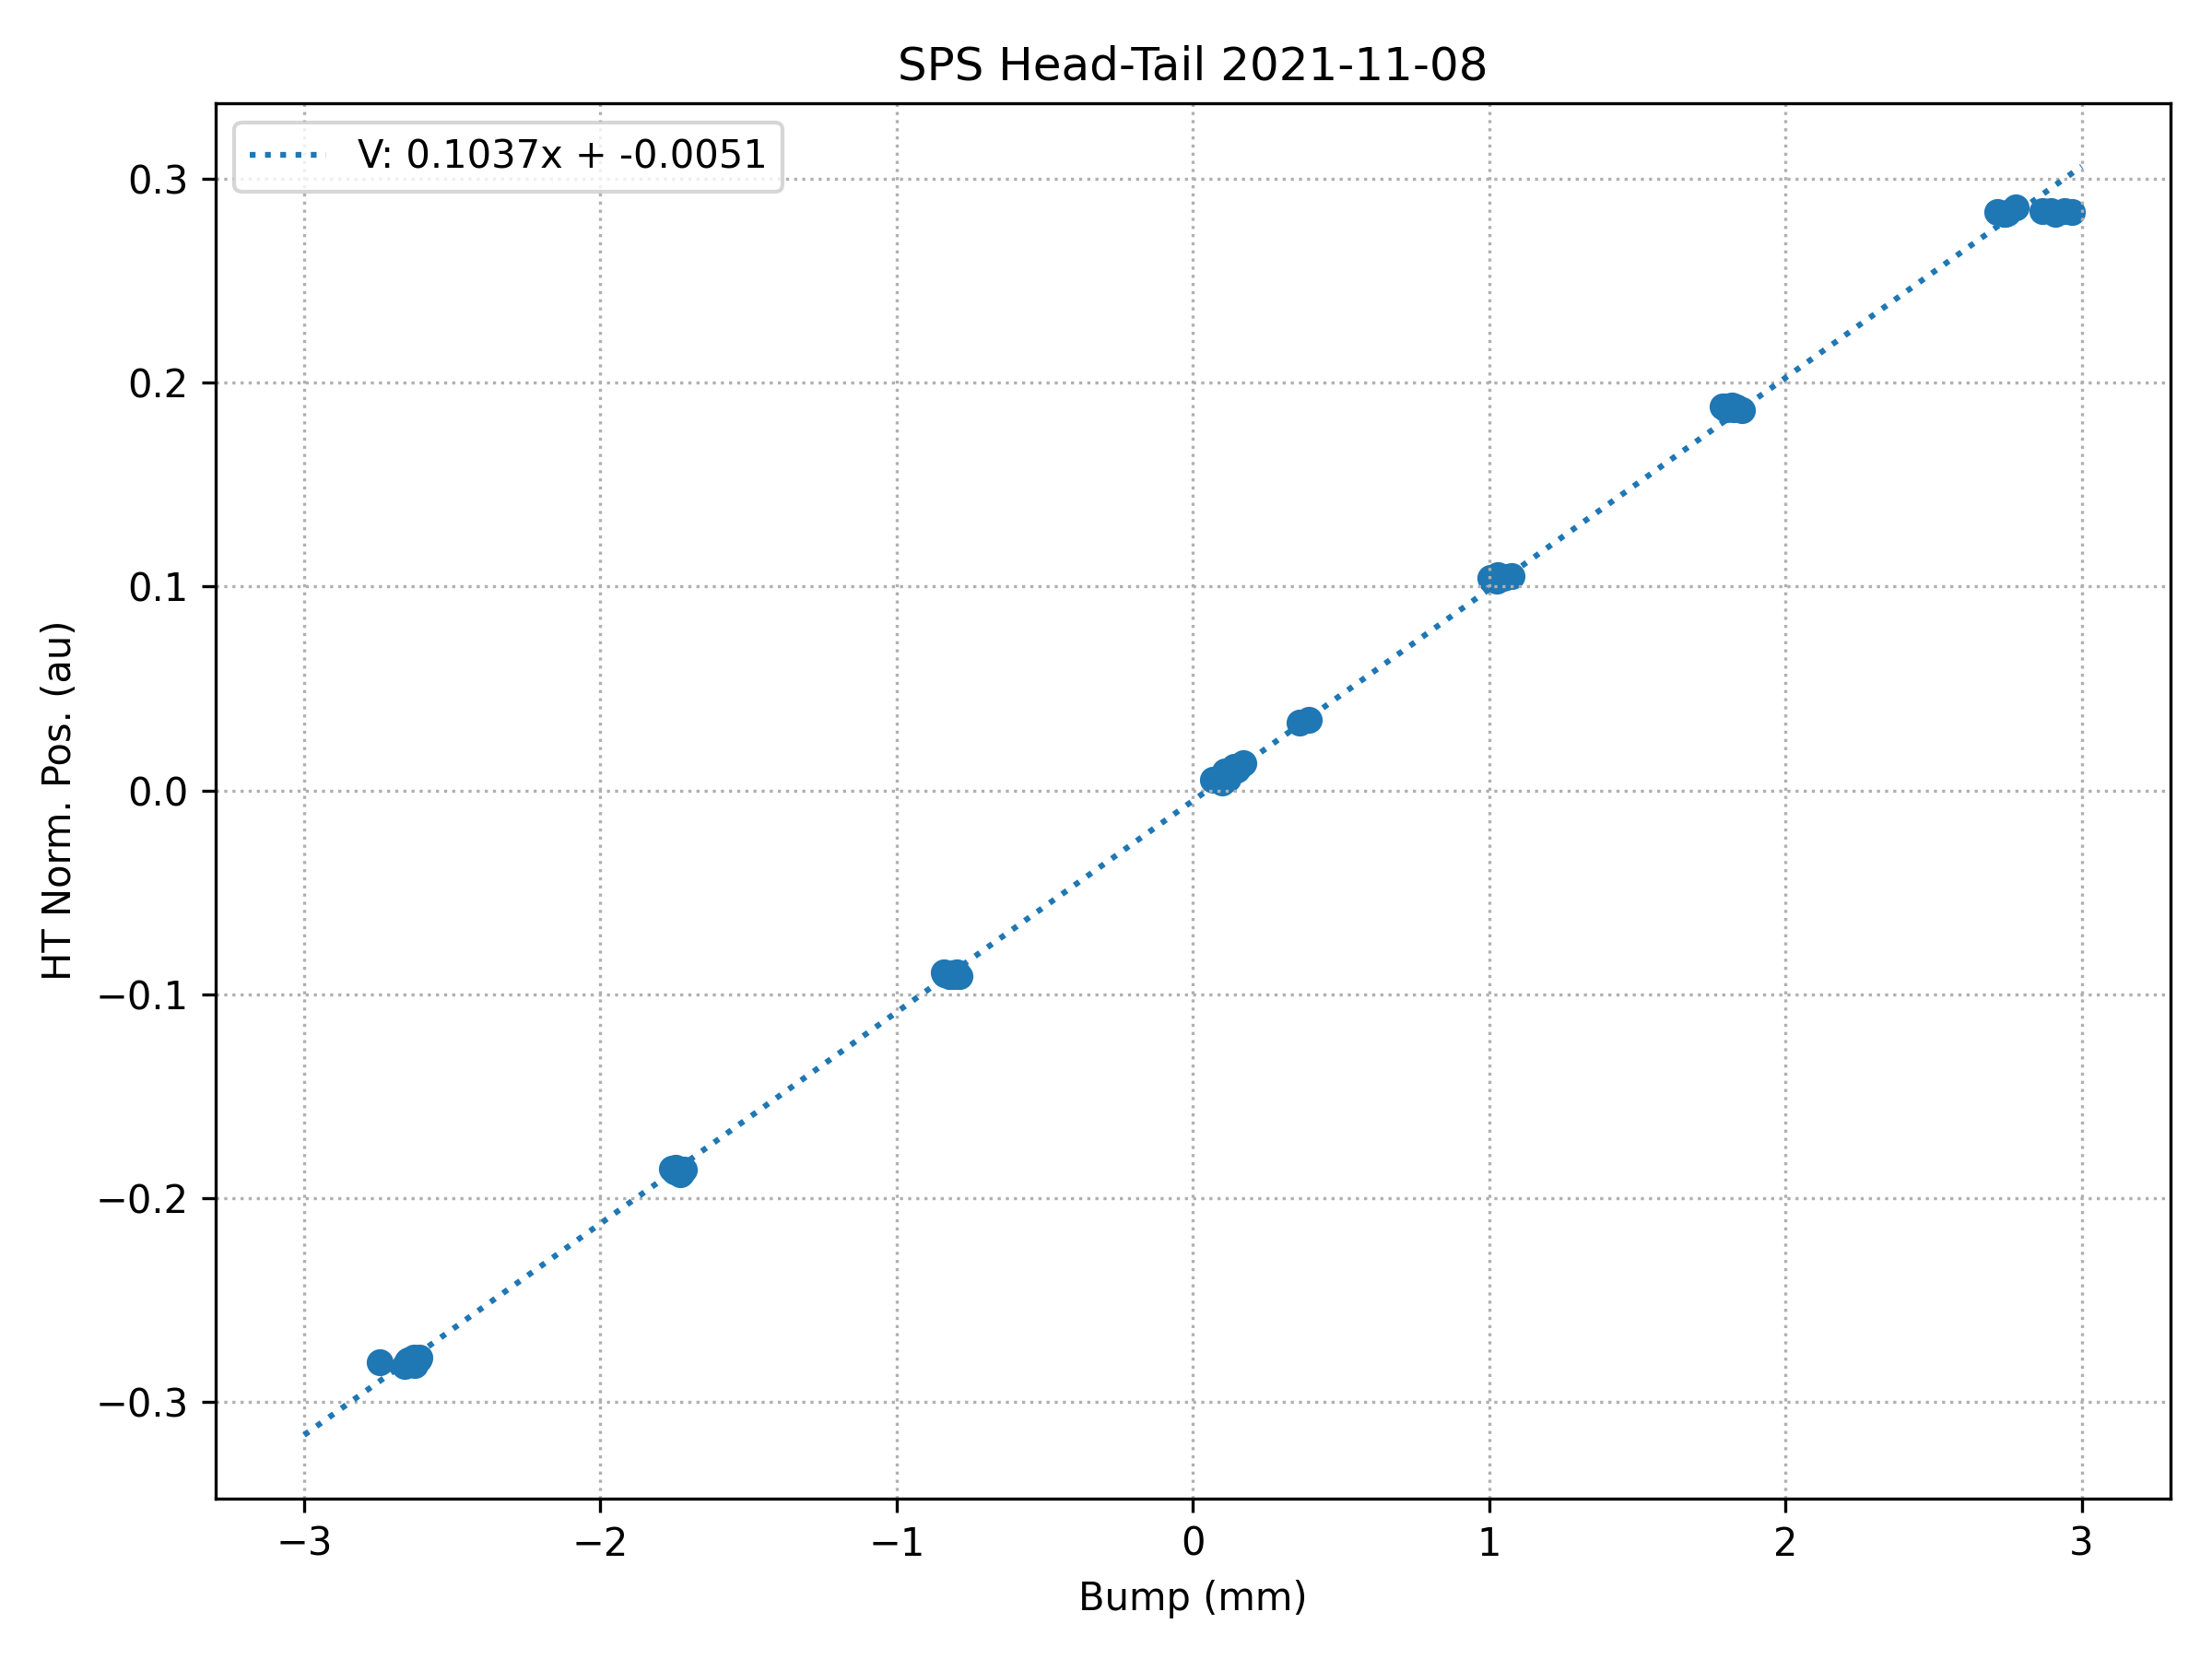
\includegraphics[width=0.7\textwidth]{images/Ch8/HT_monitor_calibration_2022.png}
%        \caption{The calibration was performed by T.~Levens by performing orbit bumps (around the reference orbit) and measuring the normalised position of the bunch in the vertical plane (plane of interest). The normalised position is obtained as the difference of the signal divided by the sum. More details on the calibration procedure are given in~\cite{PhysRevAccelBeams.22.112803}. This plot is courtesy of T.~Levens .}
%        \label{fig:HT_calibration_2022_levens}
% \end{figure}


\subsection{Experiment preparation and procedure}\label{sec:cc_md_2022_preparation}
\textbf{Objectives}\\
The available machine time ($\sim$ 10 hours) for the $\CC$ experiment of 2022 was split into two parts. For the first part, the objective was to measure the emittance growth with the same noise levels and conditions as in 2018 in order a) to reproduce the observed scaling of emittance growth (see Fig.~\ref{fig:MD5_summary_plot}) and b) to benchmark the expected suppression factor from PyHEADTAIL simulations with the impedance model. This will be referred to as $\CC$ Experiment A in the following.

The objective of the second part was to investigate the effects of impedance and amplitude detuning on the emittance growth from $\CC$ phase noise. The preceding analysis of the PyHEADTAIL simulations revealed a significant sensitivity of the emittance growth suppression on amplitude-dependent tune shift (e.g. Fig.~\ref{fig:MD_2018_impedance_simulations}). This behavior can be tested experimentally in the SPS with the use of the Landau octupole families, which allow for the introduction of controlled detuning with amplitude. A successful reproduction of this behavior would provide the proof-of-concept for the emittance growth suppression mechanism from the beam transverse impedance. This will be referred to as $\CC$ Experiment B in the following. It should be mentioned, that for this experiment the octupoles of the LOD family are employed as they act mostly in the vertical plane which is the plane of interest in this studies (vertical $\CC$ module which results in vertical emittance growth).

\textbf{Preparatory studies with PyHEADTAIL simulations}\\

\textbf{Experimental procedure}\\
The experiment was carried out on 16 May 2022, from 09:15 to 18:40. The steps taken during the experimental study were the following:

\begin{enumerate}
   \item Calibration of the $\CC$ phase offset and voltage measurement.
   \item Measurement of the background growth rate in "coast" mode: CC is switched on but with no additional noise injected in its RF system and the Landau octupoles switched off.
   \item Measurement of the emittance growth with the Landau octupoles switched off and for four different $\CC$ noise levels as in 2018 (CC Experiment A). For each noise level a new bunch was injected.
   \item Measurement of the emittance growth for a selected noise level and varying octupole strength (CC Experiment B). For each octupole setting a new bunch was injected in the SPS.
\end{enumerate}


The details and the results of the above mentioned steps will be presented in the following subsections.


\subsection{Results of CC Experiment B: sensitivity of emittance growth rates to amplitude-dependent tune shift}\label{subsec:cc_md_2022_octupole_scan}

The second part of the experiment aimed to validate that the beam coupling impedance suppresses the $\CC$ phase noise-induced emittance growth through the mechanism described in Section~\ref{sec:suppression_mechanism}. The strategy for this proof-of-concept experiment was to measure the emittance growth for one level of phase noise (-104.7\,dBc/Hz or 3.4$\times 10^{11} \ \mathrm{rad^2/Hz}$) but for different octupole settings with the goal of reproducing the behavior shown in Fig.~\ref{fig:pyheadtail_cc_impedance_2022_md_octupole_current}. In the limited time available for the experiment performing the full scan on the octupole settngs was not feasible. Only five octupole strengths could be used, $k_\mathrm{LOD} = \pm 5 \ \mathrm{m^{-4}}, 10 \ \mathrm{m^{-4}}$ and $15 \ \mathrm{m^{-4}}$. %The last value of octupole strength is expected to restore the growth rate to almost the values predicted by the Mastoridis--Baudrenghien model (approximately 20 $\mathrm{\mu m/h}$).
For each setting the bunch evolution was recorded for about 20 minutes by acquiring repeated Wire Scanner measurements and then performing a linear fit. For the measurements of each setting a fresh bunch was used so that the initial conditions each time are as close as possible.

The individual measurements of the transverse emittance evolution for each octupole setting are shown in Fig.~\ref{fig:cc_md_2022_overview_plots_klod_scan}. Two main observations can be made. First, there is a clear sensitivity of the measured evolution of the vertical emittance to the octupole strength as expected from the PyHEADTAIL simualtions with the SPS transverse impedance model. The second observation is that a growth of $\sim 2-4 \ \mathrm{\mu m/h}$ is also observed in the horizontal plane. However, it does not seem to depend on the octupole strength. Both observations are also seen in the summary plot of Fig.~\ref{fig:H_V_emit_growth_background_subtracted_octupole_scan}.

% location: /eos/user/n/natriant/2022/SPS_MDs_2022/cc_md_16May2022/roundA_online_analysis_ws/for_thesis
% script to plot: /afs/cern.ch/work/n/natriant/public/SPS_MDs_2022/cc_md_16May2022/ws_measurements 
\begin{figure}[htp]
   \centering
   \begin{subfigure}{.45\textwidth}
       \centering
       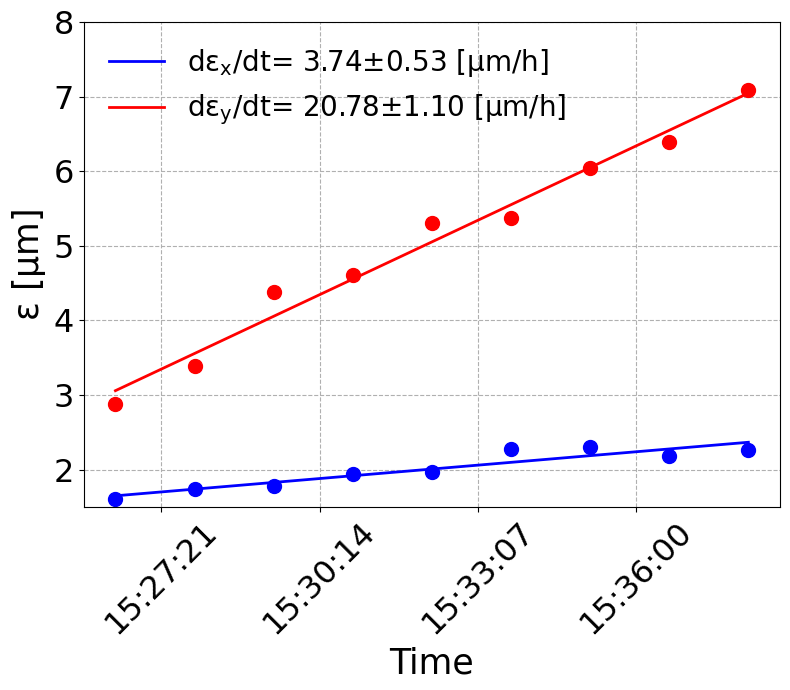
\includegraphics[width=.95\linewidth]{images/Ch8/emit_vs_time_Set1_coast6.png}  
       \caption{$k_\mathrm{LOD}=+15 \ \mathrm{/m^{4}}$}
       \label{fig:cc_md_2022_coast6}
   \end{subfigure}
   \begin{subfigure}{.45\textwidth}
       \centering
       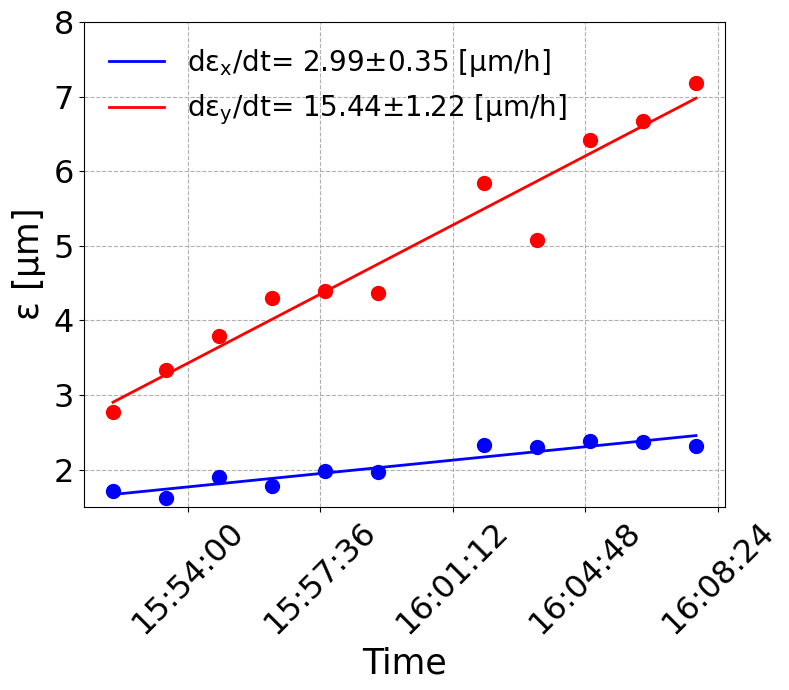
\includegraphics[width=.95\linewidth]{images/Ch8/emit_vs_time_Set1_coast7.png}  
       \caption{$k_\mathrm{LOD}=+10 \ \mathrm{/m^{4}}$}
       \label{fig:cc_md_2022_coast7}
   \end{subfigure}
   \begin{subfigure}{.45\textwidth}
       \centering
       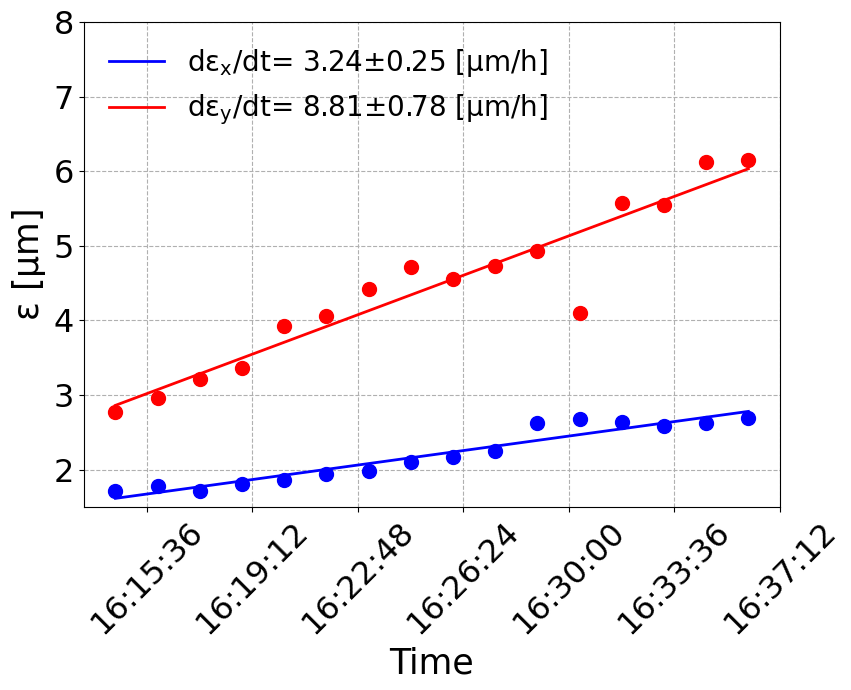
\includegraphics[width=.95\linewidth]{images/Ch8/emit_vs_time_Set1_coast8.png}  
       \caption{$k_\mathrm{LOD}=+5 \ \mathrm{/m^{4}}$}
       \label{fig:cc_md_2022_coast8}
   \end{subfigure}
   \begin{subfigure}{.45\textwidth}
           \centering
           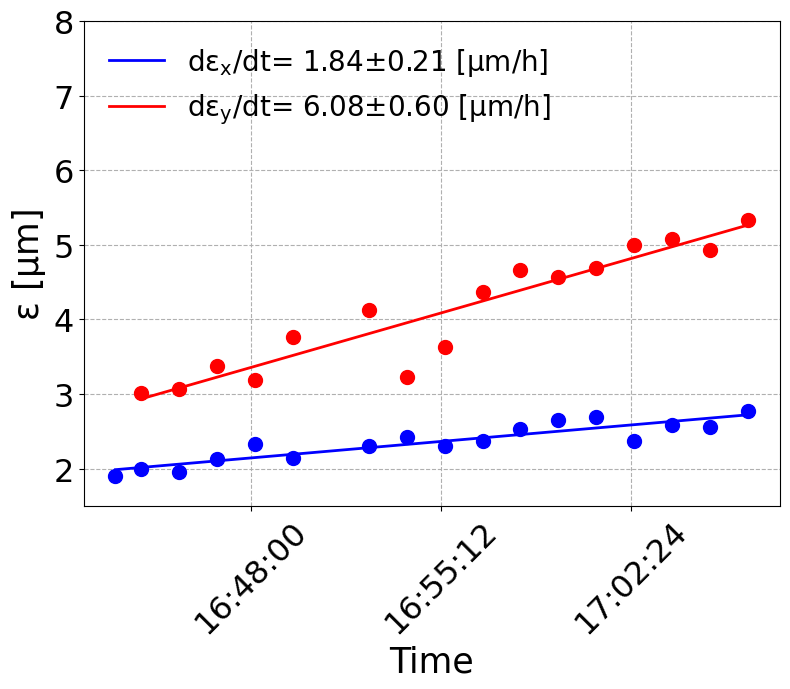
\includegraphics[width=.95\linewidth]{images/Ch8/emit_vs_time_Set1_coast9.png}  
           \caption{$k_\mathrm{LOD}=-5 \ \mathrm{/m^{4}}$}
           \label{fig:cc_md_2022_coast9}
   \end{subfigure}
   \caption{Horizontal (blue) and vertical (red) emittance evolution of a single bunch during the CC experiment on 16 May, 2022 driven by phase noise of -104.7\,dBc/Hz. The different octupole settings are displayed in the captions of each plot.}
   \label{fig:cc_md_2022_overview_plots_klod_scan}
\end{figure}

%\textbf{Unstable bunch for strong negative octupole strength}\\
Following the measurements presented above, there was an attempt to measure the emittance growth for $k_\mathrm{LOD}=-10 \ \mathrm{/m^4}$. However, the bunch was found to be unstable in the horizontal plane which resulted to loss of the beam. The instability was observed in the turn-by turn-data acquired with the base-band tune (BBQ) measurement system of SPS~\cite{Boccardi:1055568}, where the betatron oscillation amplitude appears to grow exponentially within a few seconds. This is illustrated in Fig.~\ref{fig:instability_BBQ_klod-15_4may2022}.

%The instability was first visible in the horizontal beam profiles acquired with the wire scanners, where long tails start to appear in the distribution. This is illustrated in Fig.~\ref{fig:instability_vertical_ws}. The instability was also observed in the turn-by turn-data acquired with the base-band tune (BBQ) measurement system of SPS~\cite{Boccardi:1055568}, where the betatron oscillation amplitude appears to grow exponentially within a few seconds. This is illustrated in Fig.~\ref{fig:instability_BBQ_klod-15_4may2022}.


% Screenshot from MD logbook
%\begin{figure}[!h]
%   \centering         
%   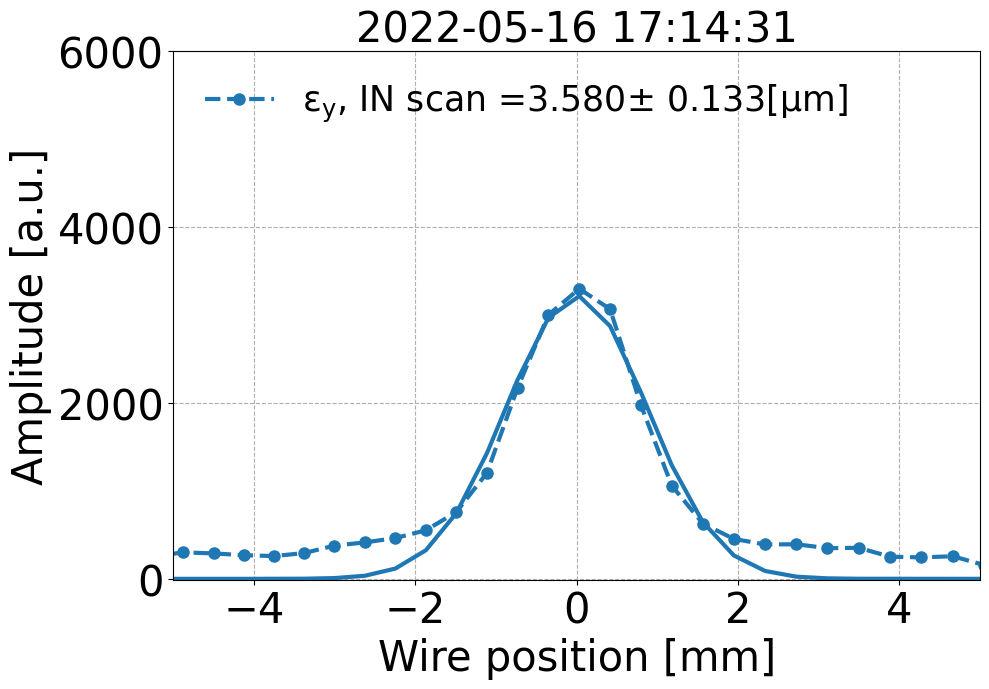
\includegraphics[width=0.7\textwidth]{images/Ch8/instability_41678.V_IN_OUT_ 17_14_31.png}
%       \caption{Example measurement of the vertical profile during the experiment with phase noise of -104.7\,dBc/Hz injected in CC1 and $k_\mathrm{LOD}=-10 \ \mathrm{/m^4}$. Due to the long tails, the Gaussian fit (solid line) does not represent well the measured points (dots connected with the dashed line).}
%       \label{fig:instability_vertical_ws}
%\end{figure}



% Figure: /eos/user/n/natriant/2022/SPS_MDs_2022/cc_md_16May2022/BBQ/figures/2022.05.16.17.49.04.430450.png
% Plotting: /eos/user/n/natriant/2022/SPS_MDs_2022/cc_md_16May2022/BBQ/plotBBQ_for_thesis.py
\begin{figure}[!h]
   \centering         
   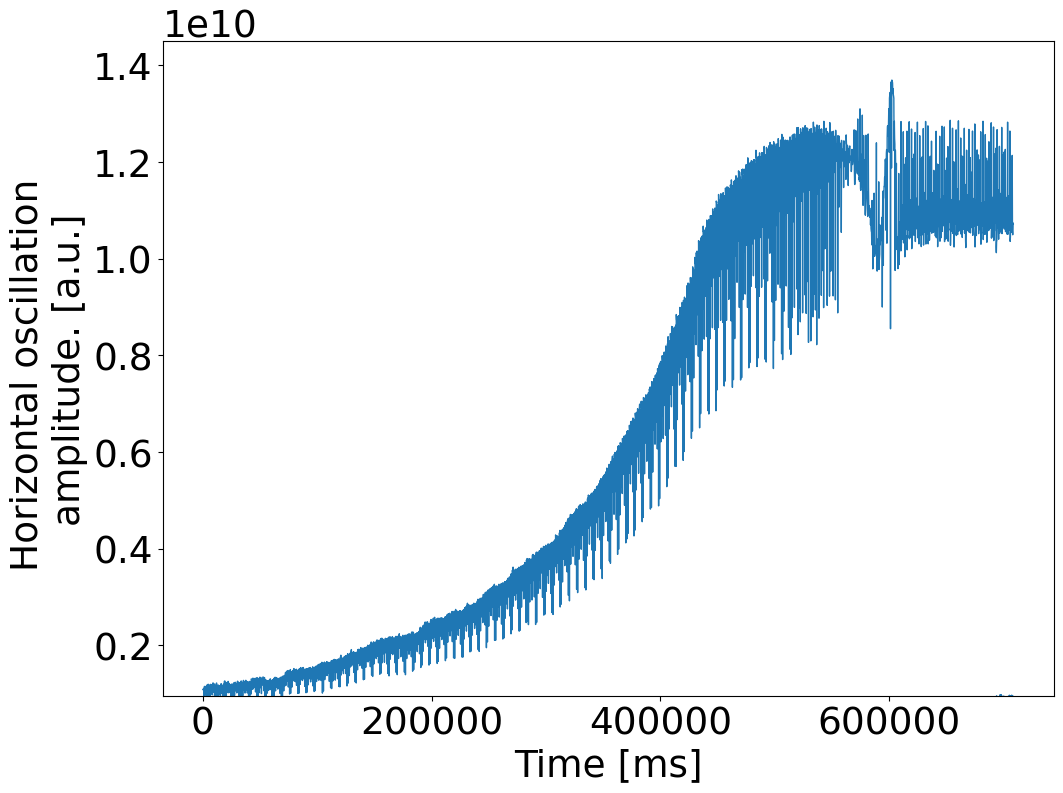
\includegraphics[width=0.7\textwidth]{images/Ch8/2022.05.16.17.49.04.430450.png}
       \caption{Example of the evolution of the horizontal oscillation of the bunch centroid during the CC measurements for $k_\mathrm{LOD}=-10 \ \mathrm{/m^4}$. This measurement is acquired with the BBQ instrument~\cite{Boccardi:1055568}.}
       \label{fig:instability_BBQ_klod-15_4may2022}
\end{figure}


The setting of almost zero linear chromaticity is the most likely explanation for this instability. As mentioned in the introduction of this chapter, the linear chromaticity was set to slightly above zero instead of 0.5-1.0 as had been requested due to miscommunication with the SPS operating team. This increased the probability of the chromaticity sliding to small negative values, which for machines like the SPS which operate above transition can result in beam instabilities~\cite{collective_effects_cas_li}.


It is worth commenting, that the instability appeared in the horizontal plane. A possible explanation is that the $k_\mathrm{LOD}$ families used for the experiment the act mainly in the vertical plane. Hence the resulted tune spread was sufficient to stabilise the beam through the mechanism of Landau damping \footnote{Landau damping is a stabilising mechanism that is applied against beam instabilities. It is demonstrated in the transverse planes in the presence of incoherent betatron tune spread. Further details can be found in~\cite{Herr:1982428, Schenk:2665819}, however a further discussion is out of the scope of this thesis.}.

\textbf{Summary plot}\\
Figure~\ref{fig:H_V_emit_growth_background_subtracted_octupole_scan} shows the measured emittance growth rates (in both planes) as functions of octupole strength. The error bars indicate the error of the linear fit on the emittance values during each coast. The background emittance growth observed in the SPS without any noise injected in the CC1 ($d\epsilon_x/dt$ = 0.81\,$\mathrm{\mu m/h}$ and $d\epsilon_y/dt$ = 0.84\,$\mathrm{\mu m/h}$) is subtracted from the measured values. 
%On this ground, it is reasonable to focus the rest of the analyisis in the vertical plane. 

Similarly to the first part of the experiment (see Section~\ref{subsec:cc_md_2022_noise_scan}), the growth in the horizontal plane seems independent of the growth in the vertical. Furthermore, Fig.~\ref{fig:H_V_emit_growth_background_subtracted_octupole_scan} shows a clear dependence of the measured vertical emittance growth rate on the octupole strengths which appears similar to that expected from the simulations. The results from the experiment support the proposed explanation (in terms of the machine impedance) for the damping of the emittance growth from $\CC$ noise.

Additionally, for the measurements with the octupoles turned off, $k_\mathrm{LOD}=0$, the suppression factor is found to be $\sim$ 4-5 which is similar to what is expected from impedance.

The measured vertical emittance growth for the large octupole strength, $k_\mathrm{LOD}$=+15\,$\mathrm{m^4}$, appears to agree with the analytical prediction of Mastoridis--Baudrenghien model. However, from PyHEADTAIL simualtions with the impedance model this behavior is expected only for octupoles stronger than 20\,$\mathrm{m^4}$ in absolute value (see Fig.~\ref{fig:pyheadtail_cc_impedance_2022_md_octupole_current}). This indicates that there is some uncertainty about the level of quantitative agreement: this will be discussed further in the following paragraph which provides a direct comparison of the measured data with the simulation results.


% appears already slightly higher than the analytical prediction. 
% Plotting script: 2022/SPS_MDs_2022/cc_md_16May2022/roundA_online_analysis_ws/summary_plots/for_thesis/cc_md_octupole_scan_for_thesis.ipynb
\begin{figure}[!h]
   \centering         
   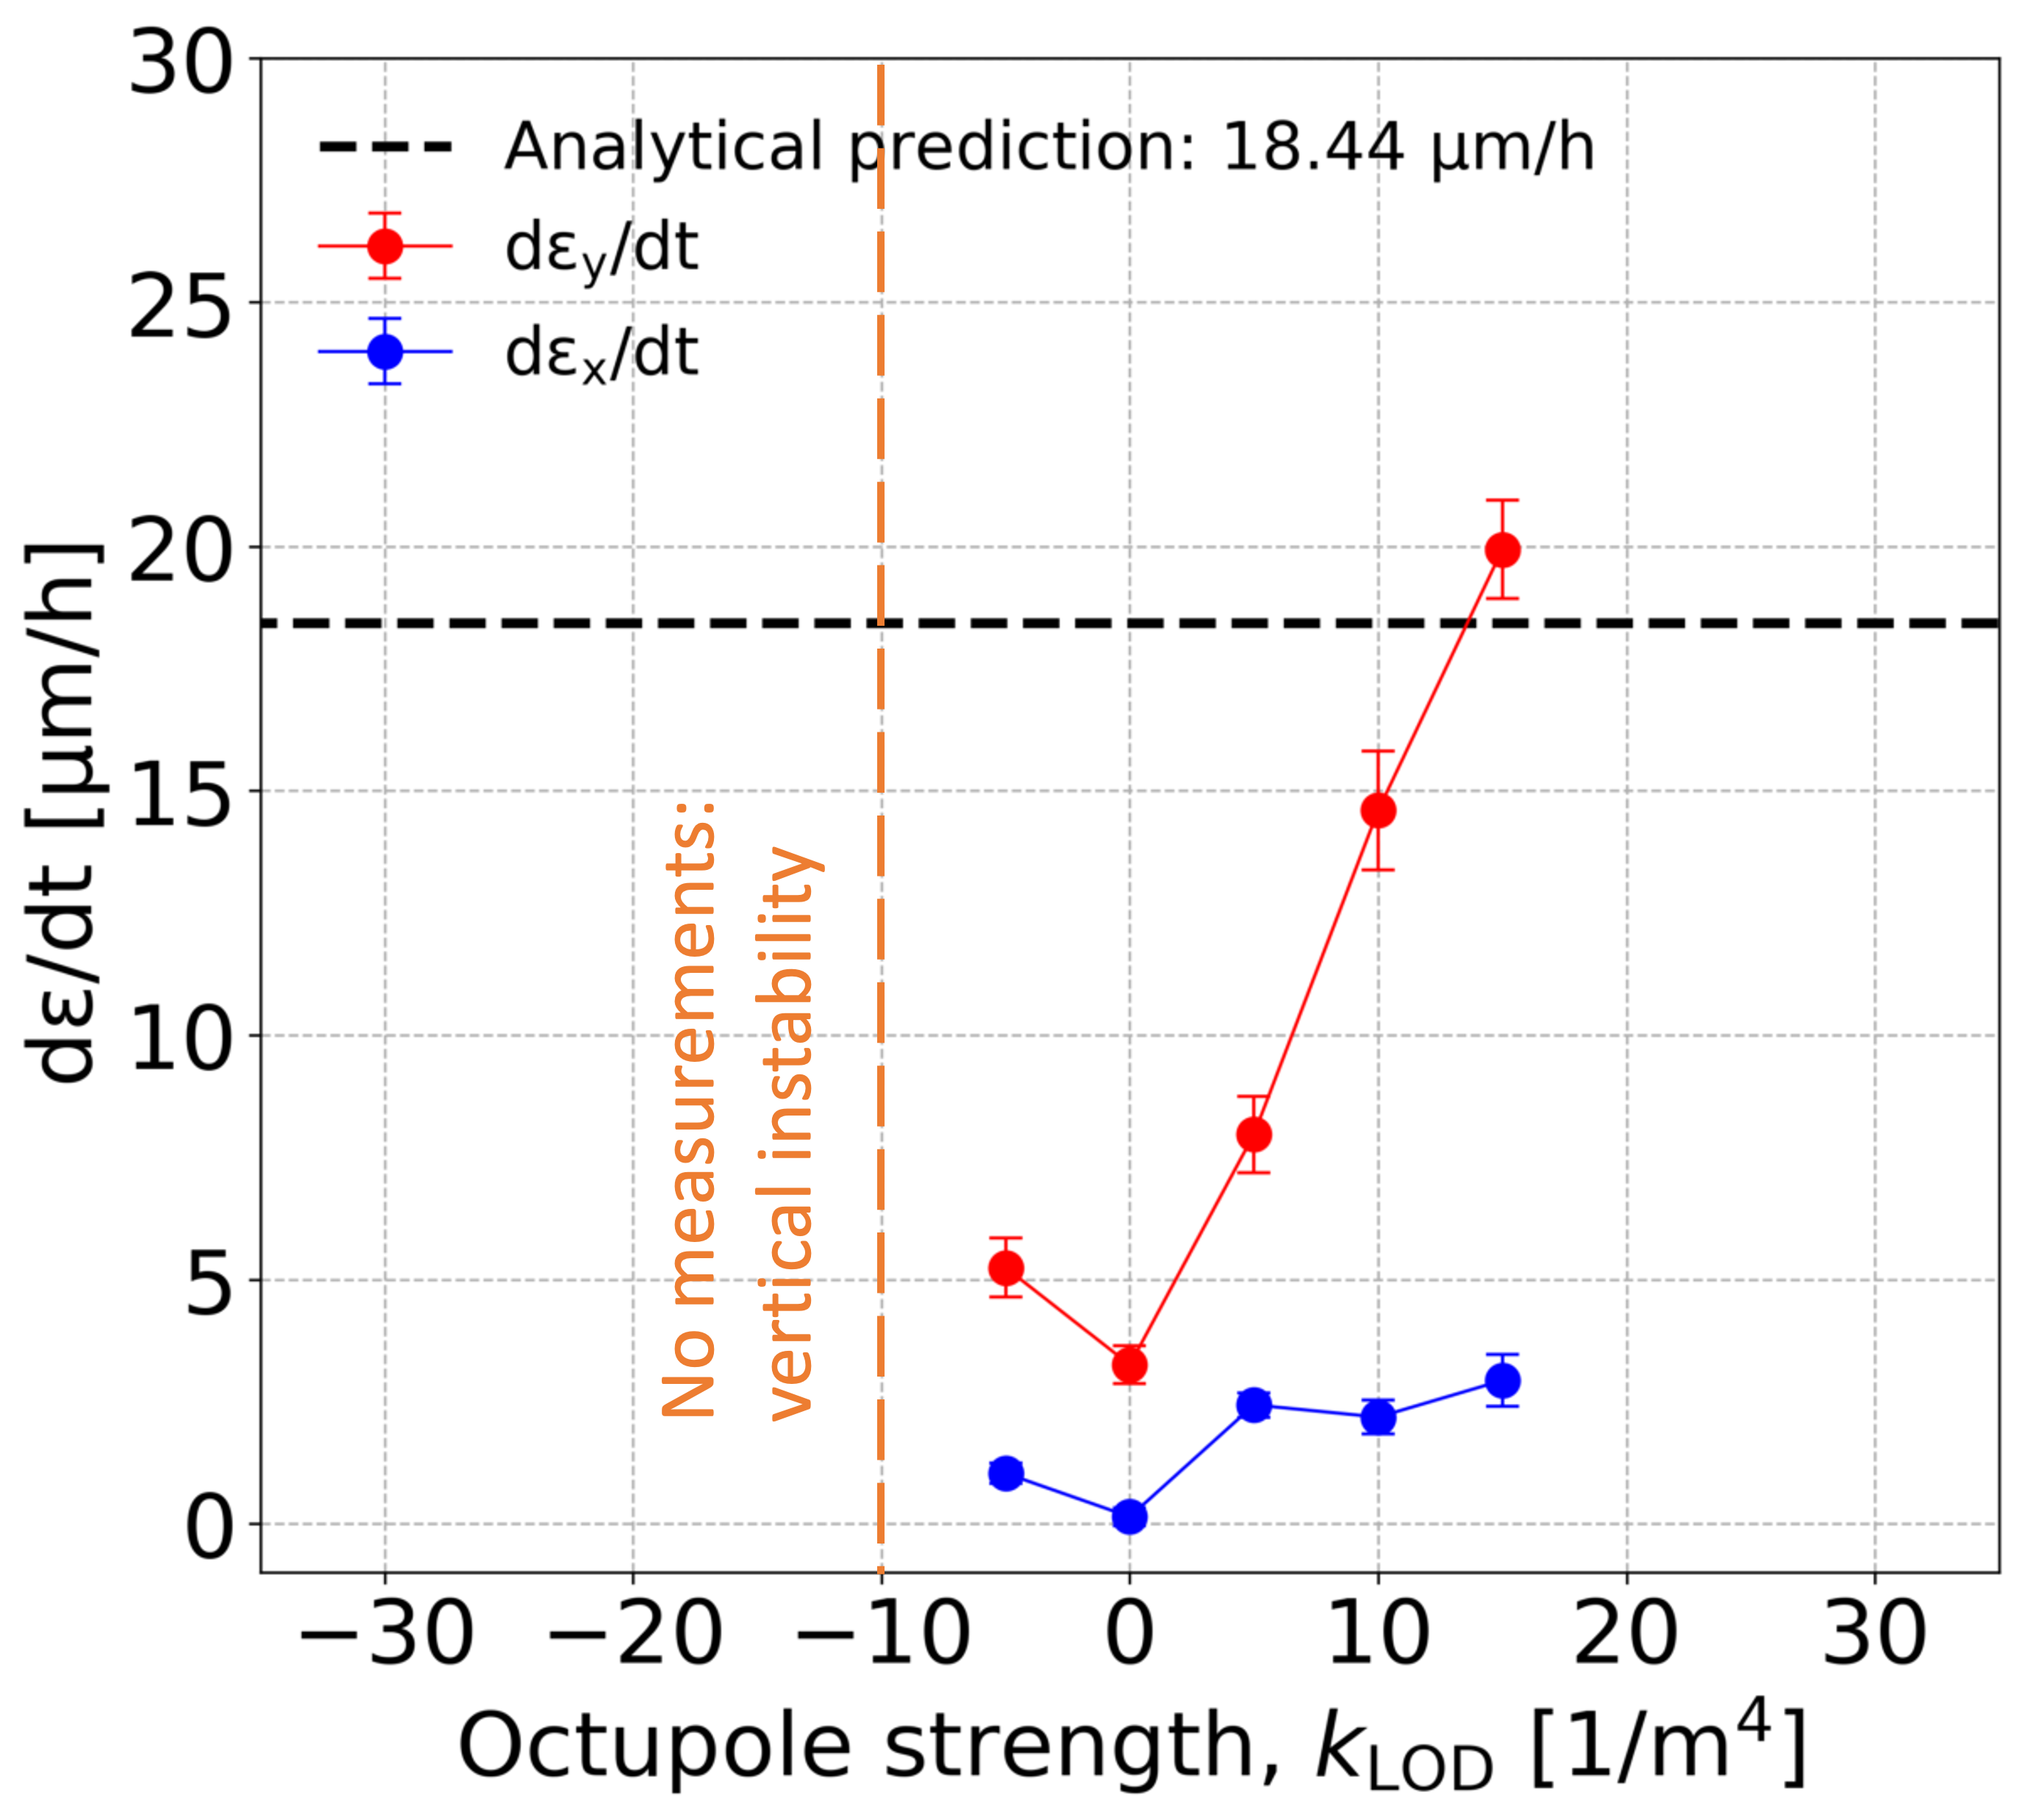
\includegraphics[width=0.7\textwidth]{images/Ch8/emit_H_and_V_octupole_scan_background_growth_subtracted_modified.png}
       \caption{Measured horizontal (blue) and vertical (red) emittance growth driven by phase noise of -104.7\,dBc/Hz injected in the RF system of CC1 for different octupole settings. The growth predicted from the analytical model without taking into account the impedance induced emittance growth suppression is $\sim$ 19\,$\mathrm{\mu m/h}$.}
       \label{fig:H_V_emit_growth_background_subtracted_octupole_scan}
\end{figure}

At this point, it should be highlighted that the degree of complexity of these studies is very high due to several reasons. First, the experiment aims to investigate the interplay of two effects: a) the $\CC$ noise-induced emittance growth and b) its suppression from impedance.  For both effects, the existing knowledge and previous experience are very limited. % for the first effect and non-existent for the second one. 
Second, preparatory studies indicated that these effects are sensitive to many parameters, including the bunch length, bunch intensity, beam energy, $\CC$ noise level, $\CC$ voltage, machine chromaticity, and tune spread. Third, a lot of uncertainties were introduced from the fact that the SPS did not operate in the usual mode. In particular, differences to the usual operational mode included the use of crab cavities, the noise injected in the CC RF system, the operation of SPS in storage ring mode, and the operation of the octupoles at unusually high strengths (requiring high currents in the coils for extended periods). % usually cycling.
Combining these factors, with the very limited machine time for the measurements, the fact that five data points were collected showing a clear dependence of emittance growth rate on octupole strength is significant.

\textbf{Comparison of measurements against PyHEADTAIL simulations with the SPS impedance}\\

Figure~\ref{fig:cc_md_2022_measurement_vs_pyheadtail_simualtion} provides a direct comparison of the vertical emittance growth measurements with the simulation results from PyHEADTAIL including the SPS transverse impedance model (discussed in Fig.~\ref{fig:pyheadtail_cc_impedance_2022_md_octupole_current}). For the comparison, both measured and simulated rates are normalised with the corresponding analytical prediction (using Eq.~\eqref{eq:dey_pn}). 

% Plotting script: /eos/user/n/natriant/pyheadtail_data/final_for_thesis/2022_conditions/CC1/normalised_growth_vs_measurements/job0010b_plot_loadFromPickles_dey_scanOverAyy_NowakesVSwakes-octupoleSettings-Noconstraintaxy_plot_normalised.ipynb
\begin{figure}[!h]
   \centering         
   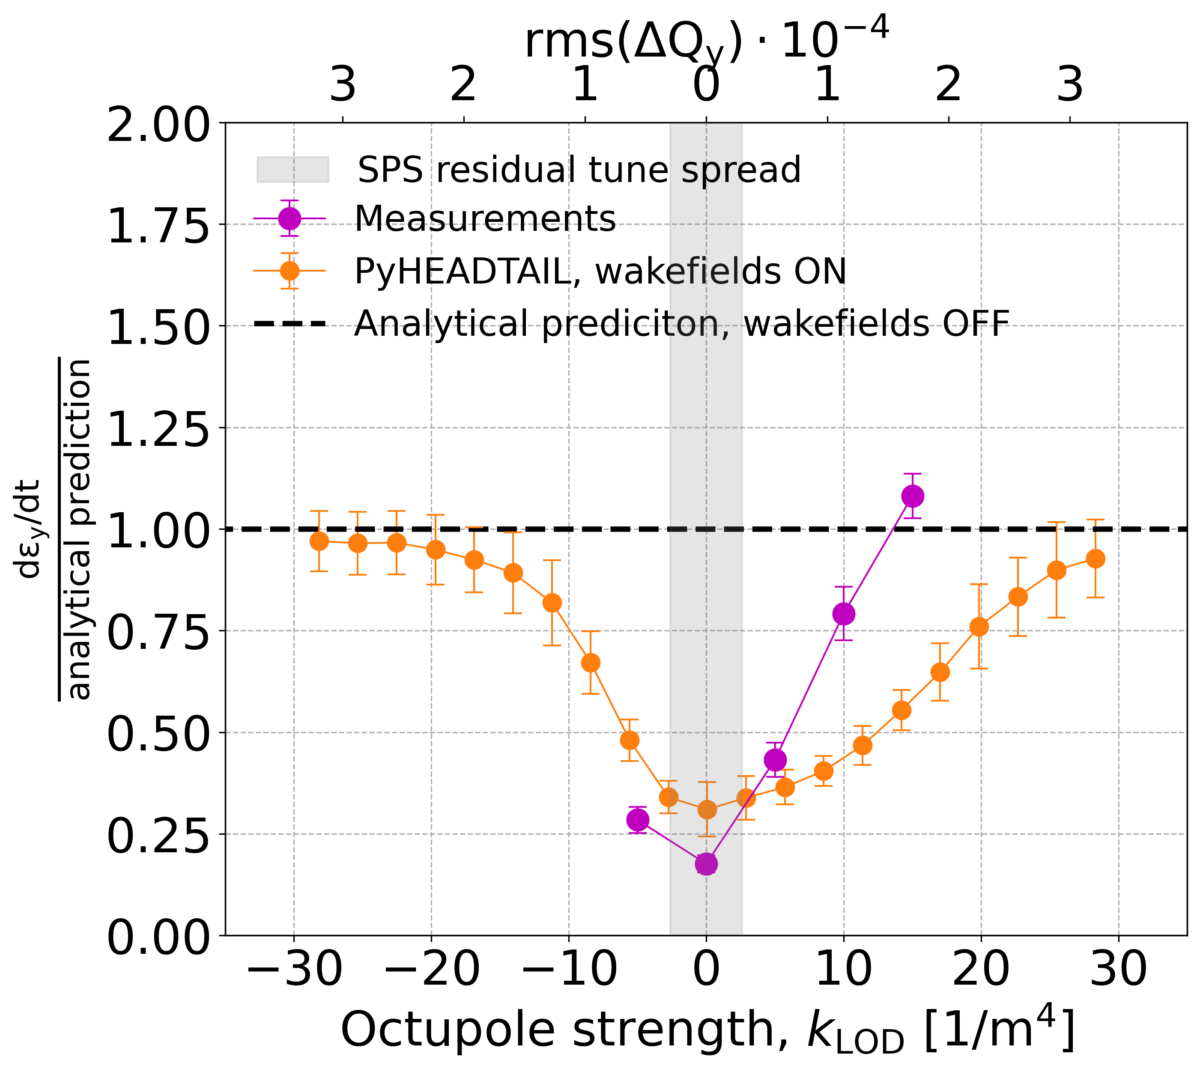
\includegraphics[width=0.7\textwidth]{images/Ch8/deyRates_sps_270GeV_PN1e-8_400MHz_SPS_NewWakesAllcontributions_appendWakes_y-plane_WakesONvsOFF_QpxQpy1_6D_Nb5e5_intensity3e10Scan_simulations_vs_measurements_magenta_new_legend.png}
       \caption{Measured (magenta) and simulated (orange) vertical emittance growth driven by phase noise injected in the RF system of CC1 for different octupole settings. Both measured and simulated rates are normalised with the corresponding prediction from the Mastoridis--Baudrenghien model.}
       \label{fig:cc_md_2022_measurement_vs_pyheadtail_simualtion}
\end{figure}

It can be seen, that there is a very good qualitative agreement of the measurements with the simulations, supporting the hypothesis that the impedance leads to damping of the emittance growth rates. Regarding the degree of quantitative agreement, there is some uncertainty, as already discussed above. Nevertheless, this is not surprising due to the complex nature of the effects, involving many different parameters, as discussed in the previous paragraph. Further studies, simulations, and measurements will be needed to investigate the quantitative agreement. One of the possible factors that could explain that quantitative agreement is not yet obtained is the contribution from space-charge: this has not yet been studied, but could affect the tune spread. Space charge was not yet taken into account as its contribution is very small for the discussed experimental configurations. Nevertheless, the tune spread values in the regime of the studies are also very small, $10^{-6}-10^{-4}$, which suggests that the space charge might play some role. This can be investigated in simulations even though it is computationally challenging.

%\begin{itemize}
%   \item The contribution from space charge which is not yet studied and it could affect the tune spread values. 
 %  \item The fact that in the experiment the vertical emittances reached significantly larger final emittances than the 2\,$\mathrm{\mu m}$ that were considered in the simulations. Larger emittances mean larger action which eventually leads to a much larger tune spread than it was initially computed for this study. In other words, for the experimental conditions, $k_\mathrm{+15} \ \mathrm{1/m^4}$ the resulting incoherent spectrum might be sufficient for the coherent tune to lie inside it. %Linear, non-linear?
%\end{itemize}

Investigations of space-charge effects may be carried out in the future, but are beyond the scope of the present work.

%As the objective of the experiment and this thesis, in general, are already achieved, these studies are considered complementary. Therefore, they are not performed yet nor they will be presented here, due to time restrictions for the completion of this thesis. 

%\subsection{Conclusions and outlook}\label{subsec:conlusions_ch8_cc_md}
%The experimental results of the additional experimental campaign with $\CC$s in SPS that took place on May 16, the year 2022 were presented in this section. The subject of the studies was the investigation of the $\CC$ noise-induced emittance growth and in particular its suppression from the beam transverse impedance. The two main objectives were a) to reproduce the scaling of the emittance growth with noise power that was observed in 2018, and b) to confirm that the beam coupling impedance can effectively suppress the $\CC$ phase noise-induced emittance growth. For the latter, the strategy was to reproduce the strong dependence of the suppression factor on the amplitude-dependent tune shift as obtained from PyHEADTAIL simulations with the SPS impedance model.

%Despite the limited available machine time and the numerous uncertainties introduced by the SPS operation outside of its usual mode, the experiment was proved successful. In particular, the experiment demonstrated that the vertical emittance increased for stronger noise in agreement with the observables of 2018 and the expectations from the available analytical model of T.~Mastoridis and P.~Baudrenghien. Moreover, the measurements showed good qualitative agreement with the expected impact of impedance and amplitude detuning: they represent a proof of concept for the mechanism of emittance growth suppression from the transverse impedance. Further studies, simulations (e.g. contribution of space charge), and measurements (e.g. varying octupole strengths over a larger range, impact of linear chromaticity, and the sensitivity to transverse instabilities), will be needed to refine the experimental observations and to investigate the quantitative agreement. 




\section{Experiment with dipole noise}\label{sec:coast_md_damper_2022}
% Presentation with the results:  https://docs.google.com/presentation/d/1C-3FPNUrUUiOFol2bdMlTqf1ZlGVamcZXjf-b4lYlUM/edit#slide=id.g1301694a1dd_0_139
The second proof-of-concept experiment to investigate the damping mechanism from the transverse impedance was conducted the night after the $\CC$ experiments described in the previous section. The emittance growth was induced by the beam damper acting as a pure dipolar noise source. This simplified the experimental procedure for two main reasons. First, there were no limitations and uncertainties introduced by the $\CC$ operation. Secondly, activating the beam damper does not require the teams which operate the $\CC$s and inject artificial noise into their RF system and thus simplifies the organisation. This mitigates the restrictions on finding an available slot for this experiment which eventually was squeezed during the night shift after the measurements with $\CC$s. % cryo team not needed

The strength of the damper kick was not calibrated and therefore the analytical expected emittance growth could not be computed. Nevertheless, the objective was to reproduce the strong dependence on the amplitude detuning which was presented in Fig.~\ref{fig:study_5_dipole_noise}. To this end, the same procedure as for the second part of the $\CC$ experiment was followed: the emittance growth was measured in "coast" mode for constant strength of the noise excitation in the vertical plane but for different octupole settings. The beam and machine parameters are summarised in Table~\ref{tab:machine_beam_param_2022}. The only update was that the linear chromaticity was corrected to $Q^\prime_{x,y}$ = 1.3 in both transverse planes to avoid instabilities due to possible shift of chromaticity to negative values (see Figs.~\ref{fig:instability_BBQ_klod-15_4may2022}).% and~\ref{fig:instability_vertical_ws}). 

The experiment lasted from about 23:50 on the May 16, 2022, until about 04:00 on the May 17, 2022. Even though the available machine time was $\sim$4 hours, only seven octupole strengths could be tested: $+25, +15, +10, +5, 0, -15, -7.5 \ \mathrm{/m^4}$. The reason is that one of the SPS quadrupole magnets tripped around 01:00 disabling the option for operation in "coast" mode, till around 03:00 when the quadrupole magnet could once more be operated.

For each octupole setting, the bunch evolution was recorded for about 10 minutes by acquiring repeated measurements with the Wire Scanners (the same instruments were used for the $\CC$ experiment earlier that day). The short duration of the measurements was a result of the strong noise excitation which resulted in a clear linear growth of the vertical emittance which quickly reached large values. This can be seen in the individual measurements of the transverse emittance evolution for each octupole setting which are presented in the Appendix~\ref{fig:emit_growth_damper_md_2022}. For the measurements of each setting a fresh bunch was injected. 

\textbf{Summary plot}\\
% no bacgkorund growth is subtracted here. It was not measured. Sensitivity very small as we are dealing with very strong emittance growth. Impact of backgorund growth is insignificant.
The experimental results are summarised in Fig.~\ref{fig:coast_dipole_noise_damper_md_2022_measurement}. The measured horizontal and vertical emittance growth are plotted as a function of the different octupole strengths with blue and red colors respectively. The error bars indicate the error of the linear fit on the emittance values during each coast. The background emittance growth without any noise excitation from the damper was not measured and thus is not subtracted from the displayed values. However, the impact of the background growth (usually measured to be between 0.5-1$\mathrm{\mu m/h}$ in both transverse planes) is insignificant for the emittance growth rates of this study ($ > 10 \ \mathrm{\mu m/m}$).
 

The emittance growth observed in the horizontal plane appears to be independent of the octupole strengths, agreeing with the observations during the $\CC$ experiment (see Section~\ref{sec:cc_md_2022}). 

In the vertical plane, there is a clear dependence of the measured emittance growth on the strength of the octupoles as expected (see Fig.~\ref{fig:study_5_dipole_noise}). The results of the experiment thus further support the hypothesis that the suppression of emittance growth observed from $\CC$ noise is a consequence of the machine impedance. However, it is not clear if the used octupole strength was sufficient to be beyond the suppression region. More data points with higher octupole strength would be needed to confirm whether this was the case, and further experiments to investigate the limits in more detail are planned. This is planned to be tested in dedicated future experiments.

Finally, it is worth commenting that, unlike the $\CC$ experiment that was conducted earlier that day, no horizontal coherent instability was observed in this experiment. It appears, that correcting to $Q^\prime_{x,y}$ = 1.3 was an effective way of avoiding it.
  

% Plotting script: /eos/user/n/natriant/2022/SPS_MDs_2022/coast_md_damper_16May2022/summary_plots/create_pickle_for_octupole_scan.ipynb
\begin{figure}[!h]
   \centering         
   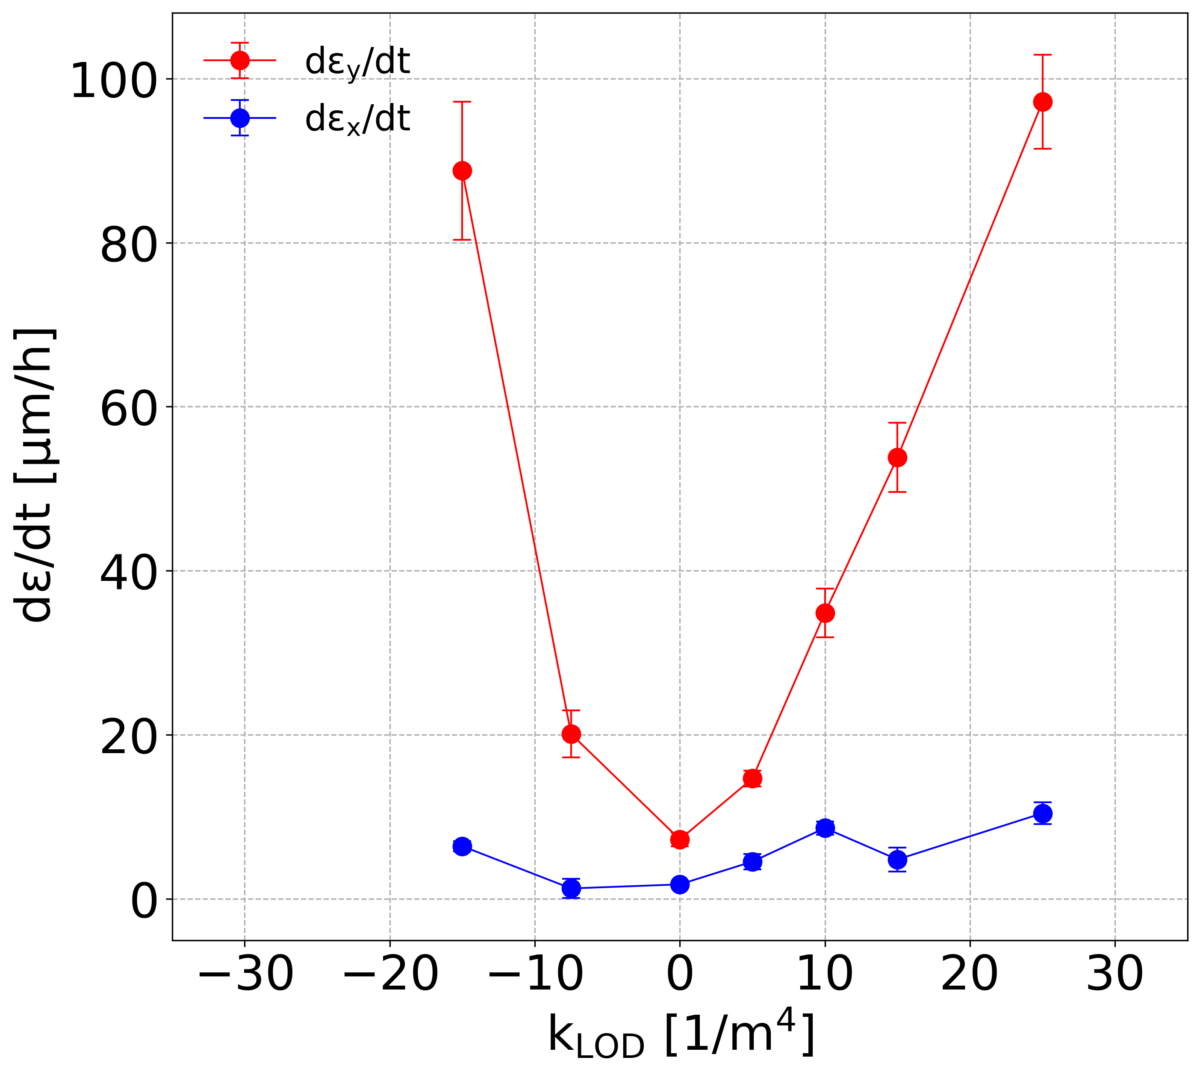
\includegraphics[width=0.7\textwidth]{images/Ch8/emitGrowth_H_V_dipole_noise_damper_md_measurements.png}
       \caption{Measured horizontal (blue) and vertical (red) emittance growth driven by dipole noise introduced with the SPS beam kicker in the vertical plane for different octupole settings.}
       \label{fig:coast_dipole_noise_damper_md_2022_measurement}
\end{figure}

\textbf{Underlying theory}\\
It is worth mentioning that the simulation studies and experimental results (from 2018 and 2022) presented in this thesis, motivated the development of a theoretical description for the suppression of the noise-induced emittance growth from the beam transverse impedance. The theory was recently developed by the colleague X.~Buffat~\cite{Buffat:2022dac, van_kamper_presentation_xavier_theory}. 

The theory developed is a simplification of the approach of Y.~Alexahin (in the context of beam-beam interactions)~\cite{Alexahin:485304}. In particular, X.~Buffat, using the Van Kampen mode approach~\cite{VANKAMPEN1955949}, adapted Y.~Alexahin's approach for configurations featuring linear detuning and a complex tune shift from a collective force. 

% This paragraph is modified from the conclusions in Xavier's paper.%
It was shown that the emittance growth driven by an external noise source can be significantly reduced by a collective force. To observe the suppression a damping force is necessary. The suppression is enhanced in configurations where the real tune shift is larger than the spread of the betatron frequencies i.e.~the coherent mode emerges from the incoherent spectrum~\cite{Buffat:2022dac}.

This theory supports the studies presented in this thesis. It also explains the asymmetry in the dependence of the emittance growth suppression for positive and negative detuning coefficients observed in PyHEADTAIL simulations (see Chapter~\ref{Ch:suppression_impedance}). Moreover, it was used to fit the experimental data measured during the experiment with dipole noise with very promising results.
% The figures is a screenshot from the plots of the following presentation: https://indico.cern.ch/event/1170242/contributions/4915101/attachments/2476586/4250387/2022-07-07_crabMD-expanded.pdf
%\begin{figure}[!h]
%   \centering         
%   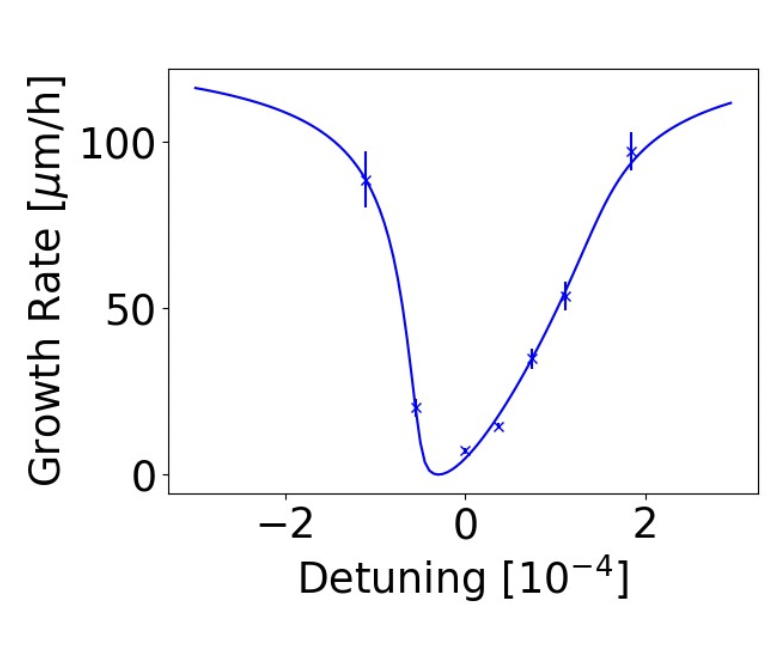
\includegraphics[width=0.6\textwidth]{images/Ch8/fit_van_kamper_damper_md_data_xavier.png}
%       \caption{Fit of Eq... to the measured emittance growth rates (points) during the experiment with a dipolar noise source. This figure is a courtesy of X.~Buffat.}
%       \label{fig:fit_van_kamper_xavier}
%\end{figure}


%\subsection{extra}
%check the  detuning with amplitude
%https://docs.google.com/presentation/d/1yaGKJ20O-jVg0R3bdj62l5VzltwjBBHtphKq5HI9xrY/edit#slide=id.g104dd3ff735_0_184


%\section{Bunch length measurements} --> Moved in the appendix
% https://docs.google.com/presentation/d/1cqXVwsXoorYqU9Td0qiFDBcyAn9XrNLmL_kvYOj61yU/edit#slide=id.g129fd6f84c7_1_5


\section{Supplementary measurements with CC RF noise}\label{sec:cc_md_Sep2022}
Due to the very promising results of the experiments that took place in May 2022 some additional machine time ($\sim$ 12 hours) was allocated for emittance growth measurements with $\CC$ RF noise on 12 September, 2022. The objective of this new round of measurements was to investigate the vertical emittance growth in the presence of $\CC$ RF phase noise and strong octupoles $|k_\mathrm{LOD} | \geq 20$\,$\mathrm{/m^4}$ for which the suppression mechanism is expected to be disabled (see Fig.~\ref{fig:pyheadtail_cc_impedance_2022_md_octupole_current}).

\subsection{Experimental setup}
The emittance growth measurements described in this section, were performed in coast mode at 270\,GeV following the same procedure with the May 2022 experiment and very similar machine and beam conditions. An overview of the paramters can be found in Table~\ref{tab:machine_beam_param_2022}. The only updated parameters were the linear chromaticity and the bunch length. In particular, the linear chromaticity was corrected to $Q^\prime_{x,y}=0.65$ in both transverse planes to ensure the coherent stability of the bunch even for large negative octupole strengths\footnote{It is reminded, that the occurance of horizontal coherent instabilities was a limiting factor in the emittance growth measurements that took place in May 2022, due to the almost zero values of linear chromaticity.}. The average bunch length (over all settings) was measured to be $4\sigma_t=1.77$\,ns. The individual plots illustrating the evolution of the bunch length for each setting during the expereiment are presented in Appendix~\ref{sec:bunch_length_measurements_sep_2022}.


\subsection{Calibration of CC phase offset and voltage measurments}
The $\CC$ calibration and the measurement of the $\CC$ voltage amplitude were performed following the procedure described in Section~\ref{subsec:cc_calibration_2022}. The results from the inspector phase scan of $\CC$1 are summarised in Fig.~\ref{fig:Vcc_calibration_md_sep2022} (blue dots).

\begin{figure}[!h] % /eos/user/n/natriant/2022/SPS_MDs_2022/cc_md_12Sep2022/HT_monitor/Vcc_at_z_zero_vs_inspector_phase_CC1_for_thesis.png
   \centering         
   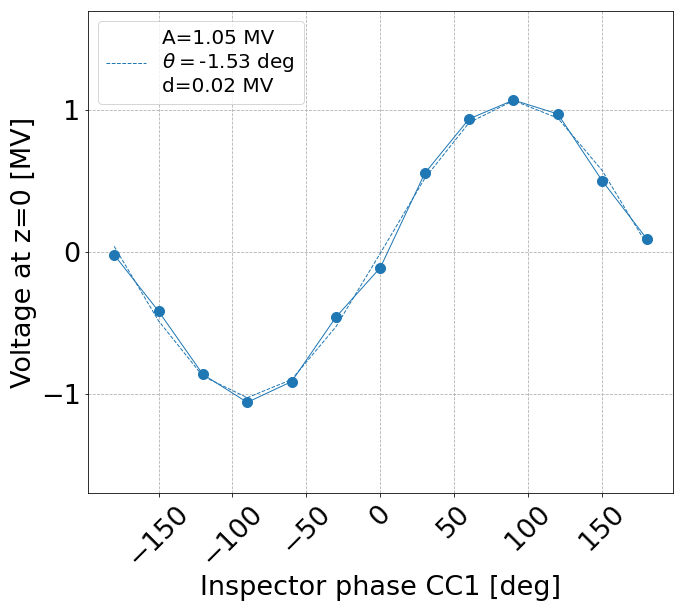
\includegraphics[width=0.7\textwidth]{images/Ch8/Vcc_at_z_zero_vs_inspector_phase_CC1_for_thesis_sep22.png}
       \caption{Calibration plot for the CC1 as obtained during the experiment on September 12, 2022, displaying the CC voltage at the center of the bunch $t=0$ for different values of the inspector phase.}
       \label{fig:Vcc_calibration_md_sep2022}
\end{figure}

The results of the sinusoidal fit of Eq.~\eqref{eq:sin_fit_cc} (blue dashed line) are given in the legend box of Fig.~\ref{fig:Vcc_calibration_md_sep2022}. From the beam-based measurements with the Head-Tail monitor the phase offset of $\CC$1 was found to be -1.54$^\circ$. For the rest of the experiment the inspector phase was set to +1.54$^\circ$ so that the phase of the $\CC$ voltage experienced by the bunch is zero. 

Tha amplitude of the $\CC$1 voltage was measured to be: $\CCvoltage=A \pm d = 1.05 \pm 0.02$\,MV very close to the targeted one of 1\,MV.

\subsection{Measurement of background growth rate in "coast" mode}
After the calibration of CC1, the coast at 270\,GeV was set up for the emittance growth measurements. First, the background transverse emittance growth, with no additional noise injected in the $\CC$ RF system, was measured. This time, the background was measured with the Landau octupoles switched ON, at $k_\mathrm{LOD}=+30$\,$\mathrm{/m^4}$. The background emittance growth was found to be: $d\epsilon_x/dt=2.42$\,$\mathrm{\mu m/h}$ and $d\epsilon_y/dt=1.62$\,$\mathrm{\mu m/h}$ in the horizontal and vertical planes respectively. The measured background emittance growth is plotted in Fig.~\ref{fig:H_V_emit_growth_background_subtracted_octupole_scan_sep22}.

%Unfortunately, there was not enough time repeat the measurement with the Landau octupoles switched off. Nevertheless, the octupoles are not expected to introduce additional tranvserse emittance growth in coast. We measured with strong octupoles to also check that the beam remain stable at large octupole strengths.

\begin{figure}[!h]
   \centering         
   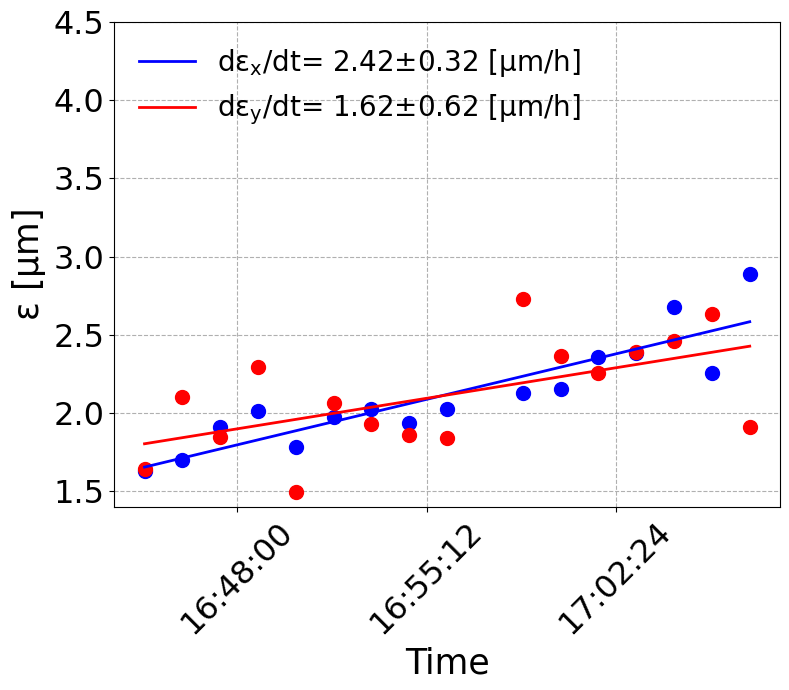
\includegraphics[width=0.7\textwidth]{images/Ch8/cc_md_12sep22_backg_coast3.png}
       \caption{Horizontal (blue) and vertical (red) background emittance growth measured during the experiment with CC1 on September 12, 2022, with no artificial noise injected in the CC RF system and with $k_\mathrm{LOD}=+30$\,$\mathrm{/m^4}$.}
       \label{fig:H_V_emit_growth_background_subtracted_octupole_scan_sep22}
\end{figure}

The background emittance growth was found to be faster than in May 16, 2022 (see Fig.~\ref{fig:cc_md_2022_background_growth_in_scan}). A possible explanation is that some growth in the transverse emittance could be driven by the operation of the Landau octupoles. Some detailed and careful investigation is required to identify the precise cause. However, due to the limited machine time, this issue should be addressed in future studies. Nevertheless, the background emittance growth is very small compared to the noise-induced emittance growth. Therefore, the non-precise knowledge of the background emittance growth does not affect the conclusions drawn from these studies. 


\subsection{Emittance growth measurements with strong octupoles}\label{subsec:cc_md_sep}
For the experiment artificial noise was injected in the RF system of $\CC1$. The noise was a mixture of both phase and amplitude noise with the phase noise being dominant. In particular, the amplitude and phase noise level at the betatron frequency were measured at -123.3\,dBc/Hz and -103.3\,dBc/Hz (slightly stronger than the phase noise used in the May experiment) respectively. From the Mastoridis--Baudrenghien model these noise levels are expected to result to a vertical emittance growth of $0.24$\,$\mathrm{\mu m/h}$ and 28.41\,$\mathrm{\mu m/h}$ respectively. These rates are computed for $\CCvoltage=1.05$\,MV and $4\sigma_t=1.77$\,ns. It is evident that the contribution of the amplitude noise to the total emittance growth is negligible hence it will not be considered in the analyisis presented in this section.

The emittance growth induced by the above mentioned RF noise was measured for five different octupole strengths, $k_\mathrm{LOD}=\pm 30, \pm 10$\,$\mathrm{/m^4}$ and $-20$\,$\mathrm{/m^4}$. The octupole strengths $| k_\mathrm{LOD} | \geq 20$\,$\mathrm{/m^4}$ are expected to restore the emittance growth rate to the values predicted by the Mastoridis--Baudrenghien model. For each octupole strength the bunch evolution was recorded for about 15-30 minures by acquiring the emittance with repeated Wire Scanner measurements and then performing a linear fit on the emittance values. For the measurements of each setting a fresh bunch was used so that the initial conditions each time were as close as possible. The measurements of the emittance evolution for each octupole strength are presented in the Appendix~\ref{sec:emit_growth_cc_md_sep2022}


Figure~\ref{fig:H_V_emit_growth_background_subtracted_octupole_scan_sep22} shows the measured horizontal (blue) and vertical (red) emittance growth as a function of octupole strength. The error bars show the error of the linear fir on the evolution of the emittance values during each setting. The background emittance growth measured without artificial noise injected in the CC1 is subtracted from the measured values. The black dashed horizontal line shows the theoretically predicted emittance growth from the Mastoridis--Baudrenghien model which does not include impedance induced effects.

% Plotting script: /eos/user/n/natriant/2022/SPS_MDs_2022/cc_md_12Sep2022/ws_emittance_growth/analysis_for_uppsala/cc_md_12Sep22.ipynb
\begin{figure}[!h]
   \centering         
   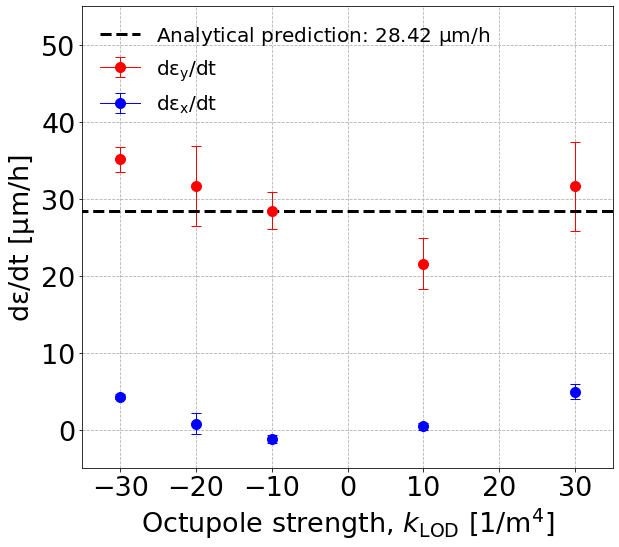
\includegraphics[width=0.7\textwidth]{images/Ch8/summary_md_12sep22_x_vs_y_backg_subtracted.png}
       \caption{Measured horizontal (blue) and vertical (red) emittance growth driven by phase noise of -103.3\,dBc/Hz injected in the RF system of CC1 for different octupole settings. The growth predicted from the analytical model without taking into account the impedance induced emittance growth suppression is $\sim$ 28\,$\mathrm{\mu m/h}$.}
       \label{fig:H_V_emit_growth_background_subtracted_octupole_scan_sep22}
\end{figure}

It is evident that the measured vertical emittance growth rates for $-30, -20$\,$\mathrm{/m^4}$ and $+30$\,$\mathrm{/m^4}$ are in agreement (within the errorbars) and they are also very close to the theoretically predicted emittance growth from the Mastoridis--Baudrenghien model, $\sim$28\,$\mathrm{\mu m /h}$. In particular, the measurements appear slightly larger than expected. However, the observed difference could be explaned by e.g. 0.1\,MV higher $\CC$ voltage\footnote{For $\CCvoltage=1.15$\,MV an emittance growth of 34$\mu m/h$ is expected from the Mastoridis--Baudrenghien model.}. An uncertainty of about 10$\%$ on the precise knowledge of the $\CC$1 voltage amplitude is reasonable.

Furthermore, the vertical emittance growth for $k_\mathrm{LOD}=-10$\,$\mathrm{/m^4}$ was measured to be larger than the rate for $k_\mathrm{LOD}=+10$\,$\mathrm{/m^4}$. This asymmetry on the emittance growth rates for positive and negative octupole strength agrees with the observables of the PyHEADTAIL simualtions which include the impedance effects (see Fig.~\ref{fig:pyheadtail_cc_impedance_2022_md_octupole_current}).

Finally, it is evident that the emittance growth in the horizontal plane increases for larger octupole strength (in absolute value). A possible explanation could be the operation of the Landau octupoles at very high currents. However, the precise source of the growth in the horizontal plane is not yet identified and further dedicated measurements are needed to provide conclusive outcome on the source of the horizontal emittance growth. 
% the coupling is corrected here. no reason to use dey+dex. This does not affect the validity of the conlsuions drawn from this study.

\subsection{Comparison of measurements against PyHEADTAIL simualations with the SPS impedance model}\label{subsec:comparison_with_pyheadtail_full_scan}
Figure~\ref{fig:cc_md_2022_measurement_vs_pyheadtail_simualtion_sep22} compares the vertical measured emittance growth with the simulation results from PyHEADTAIL including the SPS impedance model. Both measured and simulated rates are normalised with the corresponding analytical prediction. The measured emittance vertical growth is plotted from the experiments of May (magenta) and September (green) 2022.

% plotting script: /eos/user/n/natriant/pyheadtail_data/final_for_thesis/2022_conditions/CC1/normalised_growth_vs_measurements/job0010b_plot_loadFromPickles_dey_scanOverAyy_NowakesVSwakes-octupoleSettings-Noconstraintaxy_plot_normalised.ipynb
\begin{figure}[!h]
   \centering         
   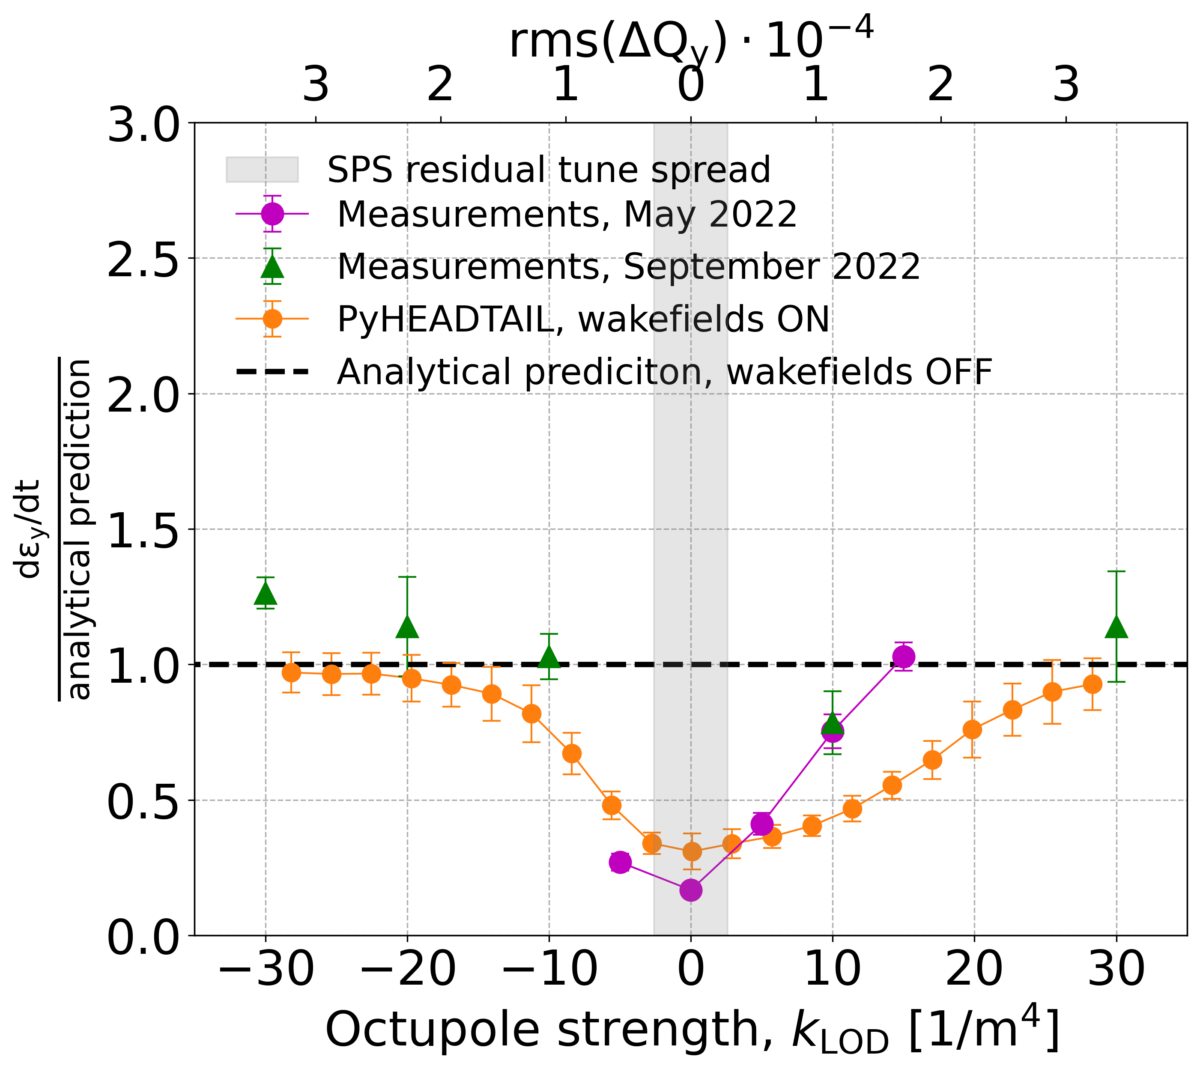
\includegraphics[width=0.7\textwidth]{images/Ch8/deyRates_sps_270GeV_PN1e-8_400MHz_SPS_NewWakesAllcontributions_appendWakes_y-plane_WakesONvsOFF_QpxQpy1_6D_Nb5e5_intensity3e10Scan_simulations_vs_measurements_magenta_new_legend_IPAC22_May_and_September_2022_for_thesis.png}
       \caption{Measured (magenta-May 2022, green-September 2022) and simulated (orange) vertical emittance growth driven by phase noise injected in the RF system of CC1 for different octupole settings. Both measured and simulated rates are normalised with the corresponding prediction from the Mastoridis--Baudrenghien model.}
       \label{fig:cc_md_2022_measurement_vs_pyheadtail_simualtion_sep22}
\end{figure}

Qualitatively, the experimental data (both from May and September) are in agreement with the simulations as they reproduce the dependence on the amplitude dependent tune spread. There is some uncertainty on the level of quantitative agreement. This could be due to various reasons which has been addressed in Sections~\ref{subsec:cc_md_2022_octupole_scan} and~\ref{subsec:cc_md_sep}.

It is worth pointing out, that the vertical emittance growth rate measured for $k_\mathrm{LOD}$=10\,$\mathrm{/m^4}$ in May was found to be in excellent agreement with the emittance growth rate measured in September for the same octupole strength. This indicates the very good reproducibility of the measurements.

\subsection{Emittance growth measurements with dominant amplitude noise}
The last 15 minutes of the available machine time were dedicated to measure the emittance growth induced by $\CC$ RF amplitude noise. 

The measurement was performed by injecting noise in the $\CC$ RF system which was a mixture of phase and amplitude noise but contrary to the experiments presented so far the amplitude noise was dominant. In particular, the amplitude and phase noise at 8\,kHz were measured to be -102\,dBc/Hz and -122\,dBc/Hz, respectively. According to Mastoridis--Baudrenghien model this noise levels should result to about 32.4\,$\mathrm{\mu m/h}$ and 0.38\,$\mathrm{\mu m/h}$, respectively. %Vcc=1.05MV, 4sigma_t = 


The emittance evolution, which was measured for $k_\mathrm{LOD}$=-30\,$\mathrm{/m^4}$, is illustrated in Fig.~\ref{fig:H_V_emit_growth_Amplitude_noise_coast12}. It can be seen that the vertical emittance growth rate, as obtained from the linear fit on the vertical emittance values (red), agrees very well with the theoretically predicted rate. This is also in agreement with the simulation results with PyHEADTAIL including the SPS impedance model (see Section~\ref{subsec:amplitude_noise}). It is reminded that in the emittance growth driven by $\CC$ RF amplitude noise is not suppressed by impedance induced effects and should be in agreement with the predictions of Mastoridis--Baudrenghien model for any value of amplitude-dependent tune spread.


% Figure: /eos/user/n/natriant/2022/SPS_MDs_2022/cc_md_12Sep2022/ws_emittance_growth/figures_for_thesis/coast12
\begin{figure}[!h]
   \centering         
   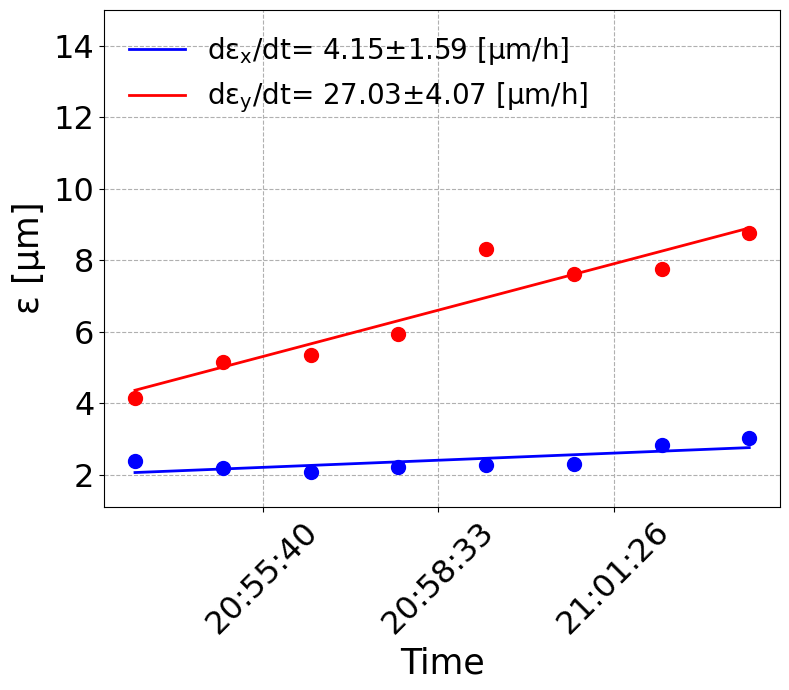
\includegraphics[width=0.6\textwidth]{images/Ch8/cc_md_sep22_AN_coast12.png}
       \caption{Horizontal (blue) and vertical (red) emittance growth measured during the experiment with CC1 on September 12, 2022}
       \label{fig:H_V_emit_growth_Amplitude_noise_coast12}
\end{figure}



\section{Conclusions and outlook}\label{sec:Ch8_conclusions}
%The experimental results of the additional experimental campaign with $\CC$s in SPS that took place on May 16, the year 2022 were presented in this section. 
In this chapter, we have summarised the results of the experiments of May and September 2022 to investigate emittance growth in SPS driven by CC phase and amplitude noise.  The main aim was to determine whether suppression of the growth rates might result from the machine impedance. The two specific objectives were a) to reproduce the scaling of the emittance growth with noise power that was observed in 2018, and b) to confirm that the beam coupling impedance can effectively suppress the $\CC$ phase noise-induced emittance growth. For the latter, the strategy was to reproduce the strong dependence of the suppression factor on the amplitude-dependent tune shift as obtained from PyHEADTAIL simulations with the SPS impedance model.

Despite the limited available machine time and the numerous uncertainties resulting from operation of the SPS outside of the usual mode, the experiment yielded useful data.. In particular, the experiment demonstrated that the vertical emittance increased for stronger noise in agreement with the observables of 2018 and the expectations from the available Mastoridis--Baudrenghien theory. Moreover, the measurements showed good qualitative agreement with the expected impact of impedance and amplitude detuning: they represent a proof of concept for the mechanism of emittance growth suppression from the transverse impedance. Further studies, simulations (e.g.~contribution of space charge), and measurements (e.g.~accuracy of beam-based measurement of $\CC$ voltage, impact of linear chromaticity, and the sensitivity to transverse instabilities), will be needed to refine the experimental observations and to investigate the quantitative agreement. 

Finally, additional measurements with emittance growth driven by a pure dipolar noise source (the beam transverse damper) clearly demonstrated the dependence of the emittance growth suppression on the amplitude-dependent tune shift.  This further supports the conclusions from the experiments using the $\CC$, regarding the hypothesis that suppression of the emittance growth can result from the machine impedance.

% From IPAC
%During the SPS CC tests in 2018, it was found that theoretical calculations of the transverse emittance growth from CC RF noise overestimated the measurements by a factor 4 (Chapter~\ref{Ch:2018_analyisis}). Simulations with PyHEADTAIL indicated that the discrepancy might be explained by impedance effects, in particular when the coherent tune is shifted outside of the incoherent spectrum (Chapter~\ref{Ch:suppression_impedance}). The simulations also indicated that the suppression is related to the dipole motion (mode 0) and a strong dependence on amplitude detuning: this was tested experimentally in the SPS in 2022. 

%The emittance growth studies took place first in the presence of $\CC$ RF phase noise and after in the presence of pure dipolar noise excitation from the beam transverse damper. The results from both expereiments show good qualitative agreement with the expected impact of impedance and amplitude detuning: they represent a proof of concept for the mechanism of emittance growth suppression from transverse impedance. 


%The noise kicks from the transverse damper were not calibrated so a quantitative comparison with the simualtion results was not feasible. For the experiment where the emittance growth was driven by $\CC$ the quantitative agreement was 


%The objective of the experimental campaign with emittance growth studies se in the SPS in 2022 was to validate experimentally the $\CC$ RF noise induced emittance growth suppression mechanism from the beam transverse impedance as suggested by PyHEADTAIL simualtions. The simualtions suggested that the meachanism is related to the dipole motion (mode 0) to this end two experiments took place. In the first, the emittance growth was driven by $\CC$ RF phase noise (like in 2018), while in the second it was driven by the beam transverse noise which provided a pure dipolar noise excitation.

%This would a) explain the 

%IPAC?

